\documentclass[a4paper,11pt]{book}
%\documentclass[a4paper,twoside,11pt,titlepage]{book}
\usepackage{listings}
\usepackage[utf8]{inputenc}
\usepackage[spanish]{babel}

\usepackage{glossaries}
%\usepackage{titlesec}
%\usepackage{pailatino}
% Para el uso de FloatBarrier
\usepackage{placeins}

% Para ajustar 
\usepackage{adjustbox}
\usepackage{multicol}

% Para la representación de tablas
\usepackage{tabularx}
\usepackage{multirow}
\usepackage{booktabs}
\usepackage[table,xcdraw]{xcolor}

\newcommand{\mc}[3]{\multicolumn{#1}{#2}{#3}}
\newcommand{\mr}[3]{\multirow{#1}{#2}{#3}}
\newcommand{\nl}{\tabularnewline}

% Para la realización de digramas de gantt
\usepackage{pgfgantt}
\usepackage[spanish]{datetime2}
\usepackage{pgfcalendar}

\renewcommand*{\pgfcalendarmonthname}[1]{%
  \ifcase#1\or
  enero\or febrero\or marzo\or abril\or mayo\or junio\or
  julio\or agosto\or septiembre\or octubre\or noviembre\or diciembre\fi
}

% Para la representación de esquemas
\usepackage{tikz}
\usetikzlibrary{positioning, arrows}

 % PARA CODIGO PYTHON
\usepackage{listings}

\lstdefinestyle{mybash}{
    language=bash,
    breaklines=true,
    basicstyle=\ttfamily\small,
    keywordstyle=\color{blue},
    stringstyle=\color{red},
    commentstyle=\color{olive},
    morecomment=[l]{\#},
    morekeywords={screen, ifconfig, ovs-vsctl, sshpass, ssh, ovsdb-server, ovs-vswitchd},
    emph={then, do, done, fi, for, if, in},
    emphstyle={\color{blue}},
    identifierstyle=\color{black},
    numberstyle=\tiny\color{gray},
    frame=single,
    backgroundcolor=\color{white}
}

\lstdefinestyle{mypy}{
    language=Python,
    breaklines=true,
    basicstyle=\ttfamily,
    keywordstyle=\color{blue},
    stringstyle=\color{red},
    commentstyle=\color{green},
    morecomment=[l]{\#},
}


\decimalpoint
\usepackage{dcolumn}
\newcolumntype{.}{D{.}{\esperiod}{-1}}
\makeatletter
\addto\shorthandsspanish{\let\esperiod\es@period@code}
\makeatother


%\usepackage[chapter]{algorithm}
\RequirePackage{verbatim}
%\RequirePackage[Glenn]{fncychap}
\usepackage{fancyhdr}
\usepackage{graphicx}
\usepackage{afterpage}

\usepackage{longtable}

\usepackage[pdfborder={000}]{hyperref} %referencia

% ********************************************************************
% Re-usable information
% ********************************************************************
\newcommand{\myTitle}{Título del proyecto\xspace}
\newcommand{\myDegree}{Grado en ...\xspace}
\newcommand{\myName}{Nombre Apllido1 Apellido2 (alumno)\xspace}
\newcommand{\myProf}{Nombre Apllido1 Apellido2 (tutor1)\xspace}
\newcommand{\myOtherProf}{Nombre Apllido1 Apellido2 (tutor2)\xspace}
%\newcommand{\mySupervisor}{Put name here\xspace}
\newcommand{\myFaculty}{Escuela Técnica Superior de Ingenierías Informática y de
Telecomunicación\xspace}
\newcommand{\myFacultyShort}{E.T.S. de Ingenierías Informática y de
Telecomunicación\xspace}
\newcommand{\myDepartment}{Departamento de ...\xspace}
\newcommand{\myUni}{\protect{Universidad de Granada}\xspace}
\newcommand{\myLocation}{Granada\xspace}
\newcommand{\myTime}{\today\xspace}
\newcommand{\myVersion}{Version 0.1\xspace}


\addto\captionsspanish{
  \renewcommand{\listtablename}{Índice de tablas}
  \renewcommand{\tablename}{Tabla}
}


\hypersetup{
pdfauthor = {\myName (email (en) ugr (punto) es)},
pdftitle = {\myTitle},
pdfsubject = {},
pdfkeywords = {palabra_clave1, palabra_clave2, palabra_clave3, ...},
pdfcreator = {LaTeX con el paquete ....},
pdfproducer = {pdflatex}
}

%\hyphenation{}


%\usepackage{doxygen/doxygen}
%\usepackage{pdfpages}
\usepackage{url}
\usepackage{colortbl,longtable}
\usepackage[stable]{footmisc}
%\usepackage{index}

\renewcommand{\tablename}{Tabla}
%\usepackage[style=long, cols=2,border=plain,toc=true,number=none]{glossary}
% \makeglossary

% Definición de comandos que me son tiles:
%\renewcommand{\indexname}{Índice alfabético}
%\renewcommand{\glossaryname}{Glosario}

\pagestyle{fancy}
\fancyhf{}
\fancyhead[LO]{\leftmark}
\fancyhead[RE]{\rightmark}
\fancyhead[RO,LE]{\textbf{\thepage}}
\renewcommand{\chaptermark}[1]{\markboth{\textbf{#1}}{}}
\renewcommand{\sectionmark}[1]{\markright{\textbf{\thesection. #1}}}

\setlength{\headheight}{1.5\headheight}

\newcommand{\HRule}{\rule{\linewidth}{0.5mm}}
%Definimos los tipos teorema, ejemplo y definición podremos usar estos tipos
%simplemente poniendo \begin{teorema} \end{teorema} ...
\newtheorem{teorema}{Teorema}[chapter]
\newtheorem{ejemplo}{Ejemplo}[chapter]
\newtheorem{definicion}{Definición}[chapter]

\definecolor{gray97}{gray}{.97}
\definecolor{gray75}{gray}{.75}
\definecolor{gray45}{gray}{.45}
\definecolor{gray30}{gray}{.94}

\lstset{ frame=Ltb,
     framerule=0.5pt,
     aboveskip=0.5cm,
     framextopmargin=3pt,
     framexbottommargin=3pt,
     framexleftmargin=0.1cm,
     framesep=0pt,
     rulesep=.4pt,
     backgroundcolor=\color{gray97},
     rulesepcolor=\color{black},
     %
     stringstyle=\ttfamily,
     showstringspaces = false,
     basicstyle=\scriptsize\ttfamily,
     commentstyle=\color{gray45},
     keywordstyle=\bfseries,
     %
     numbers=left,
     numbersep=6pt,
     numberstyle=\tiny,
     numberfirstline = false,
     breaklines=true,
   }
 
% minimizar fragmentado de listados
\lstnewenvironment{listing}[1][]
   {\lstset{#1}\pagebreak[0]}{\pagebreak[0]}

\lstdefinestyle{CodigoC}
   {
	basicstyle=\scriptsize,
	frame=single,
	language=C,
	numbers=left
   }
\lstdefinestyle{CodigoC++}
   {
	basicstyle=\small,
	frame=single,
	backgroundcolor=\color{gray30},
	language=C++,
	numbers=left
   }

 
\lstdefinestyle{Consola}
   {basicstyle=\scriptsize\bf\ttfamily,
    backgroundcolor=\color{gray30},
    frame=single,
    numbers=none
   }


\newcommand{\bigrule}{\titlerule[0.5mm]}





%Para conseguir que en las páginas en blanco no ponga cabecerass
\makeatletter
\def\clearpage{%
  \ifvmode
    \ifnum \@dbltopnum =\m@ne
      \ifdim \pagetotal <\topskip
        \hbox{}
      \fi
    \fi
  \fi
  \newpage
  \thispagestyle{empty}
  \write\m@ne{}
  \vbox{}
  \penalty -\@Mi
}
\makeatother

\usepackage{pdfpages}
\usepackage{appendix}
\usepackage{float}
\usepackage[utf8]{inputenc}
\usepackage[nottoc,notlof,notlot]{tocbibind}
\usepackage{rotating}
\usepackage{microtype}
\usepackage[T1]{fontenc}
\usepackage{longtable} % para tablas largas
\usepackage{tabulary}
\usepackage{listings}
\usepackage{xcolor} % Para colores personalizados

\lstset{
  basicstyle=\ttfamily\small,
  columns=fullflexible,
  frame=single, % Marco alrededor del código
  breaklines=true,
  postbreak=\mbox{\textcolor{red}{$\hookrightarrow$}\space},
  showstringspaces=false, % No mostrar espacios en strings
  % numbers=left, % Eliminar o comentar para quitar los números de línea
  numberstyle=\tiny, % Estilo de los números de línea
  numbersep=5pt, % Distancia de los números de línea al código
  xleftmargin=0.2cm, % Reducir para aumentar el ancho del recuadro
  xrightmargin=0.2cm, % Reducir para aumentar el ancho del recuadro
  captionpos=b % Posición de la leyenda (bottom)
}
\begin{document}

    % RODGOM - INCLUYO ESTO PARA LA NUMERACIÓN CORRECTA
    \frontmatter
    % Plantilla portada UGR
    \begin{titlepage}
 
 
\newlength{\centeroffset}
\setlength{\centeroffset}{-0.5\oddsidemargin}
\addtolength{\centeroffset}{0.5\evensidemargin}
\thispagestyle{empty}

\noindent\hspace*{\centeroffset}\begin{minipage}{\textwidth}

\centering

\includegraphics[width=0.9\textwidth]{imagenes/logo_ugr.jpg}\\[1.4cm]

\textsc{ \Large TRABAJO FIN DE GRADO\\[0.2cm]}
\textsc{GRADO EN INGENIERÍA INFORMÁTICA}\\[1cm]
% Upper part of the page
% 
% Title
{\Huge\bfseries  Sistema de Tutorización Inteligente para la Enseñanza de Programación a Niños\\[0.2cm]}
\noindent\rule[-1ex]{\textwidth}{3pt}\\[3.5ex]
{\large\bfseries Diseño e Implementación de una Plataforma Web con un Sistema de Tutorización Inteligente para facilitar la Enseñanza}
\end{minipage}

\vspace{0.5cm}
\noindent\hspace*{\centeroffset}\begin{minipage}{\textwidth}
\centering

\textbf{Autor}\\ {Noelia Carrasco Vilar}\\[1cm]
\textbf{Director}\\ {José Manuel Benítez Sánchez}\\[1cm]

\includegraphics[width=0.3\textwidth]{imagenes/etsiit_logo.png}\\[0.5cm]
\textsc{Escuela Técnica Superior de Ingenierías Informática y de Telecomunicación}\\
\textsc{---}\\
Granada, Noviembre de 2023
\end{minipage}
\end{titlepage}

    
    

    % Plantilla prefacio UGR
    \chapter*{}
\thispagestyle{empty}
\begin{center}

\large\bfseries Sistema de Tutorización Inteligente para la Enseñanza de Programación a Niños\\[1cm]

\end{center}

\begin{center}

Noelia Carrasco Vilar \\

\end{center}

\vspace{0.5cm}
\noindent{\textbf{Palabras clave}:
\textit{Sistema de Tutorización Inteligente},
\textit{Educación Infantil},
\textit{Análisis},
\textit{Automatización},
\textit{Programación}}
\vspace{0.5cm}

\noindent{\textbf{Resumen}}\\

La enseñanza de la programación en edades tempranas se ha vuelto fundamental en la sociedad actual. Es en este contexto donde los Sistemas de Tutorización Inteligente (ITS) emergen como herramientas potenciales para apoyar un aprendizaje más personalizado y adaptado a las necesidades individuales de cada estudiante.

Este trabajo presenta el diseño, desarrollo y evaluación de un ITS enfocado en la enseñanza de programación. El sistema propuesto aplica una automatización en la corrección de los ejercicios con tal de poder ofrecer una buena retroalimentación en tiempo real. Además de adaptarse a las necesidades individuales de los estudiantes y monitorizar su progreso. 

El proceso de desarrollo del ITS se llevó a cabo en diversas fases. En primer lugar, se establecieron los fundamentos pedagógicos y se identificaron las necesidades específicas del público infantil. Posteriormente, se integraron técnicas avanzadas de corrección y elección de ejercicios con tal de garantizar la adaptabilidad y efectividad del sistema.

Para evaluar la eficacia, se realizó una prueba con un pequeño grupo de estudiantes, en colaboración con la empresa CODELEARN S.L. Los resultados iniciales sugirieron una posible mejora en la retención de conocimientos y en el rendimiento académico de los participantes, validando así la propuesta de este TFG.

En conclusión, este Trabajo de Fin de Grado aporta una solución innovadora al campo de la educación tecnológica infantil, demostrando la viabilidad y eficacia de los Sistemas de Tutorización Inteligente dentro del mundo educativo de la programación más allá de la corrección rutinaria.


% ABSTRACT

\chapter*{}
\thispagestyle{empty}

\begin{center}

{\large\bfseries Intelligent Tutoring System for Teaching Programming to Children}\\[1cm]

\end{center}

\begin{center}

Noelia Carrasco Vilar\\

\end{center}

\vspace{0.5cm}
\noindent{\textbf{Keywords}:
\textit{Intelligent Tutoring System},
\textit{Early Childhood Education},
\textit{Analysis},
\textit{Automation},
\textit{Programming}}
\vspace{0.5cm}

\noindent{\textbf{Abstract}}\\

Teaching programming at an early age has become essential in today's society. It is in this context that Intelligent Tutoring Systems (ITS) emerge as potential tools to support more personalized learning tailored to the individual needs of each student.

This work presents the design, development, and evaluation of an ITS focused on teaching programming to children. The proposed system applies automation techniques in exercise correction to provide real-time feedback on the student's understanding. It is also capable of adapting to individual student needs and monitoring their progress.

The development of the ITS was carried out in various phases. Firstly, pedagogical foundations were established, and the specific needs of the child audience were identified. Advanced correction and exercise selection techniques were then integrated to ensure the adaptability and effectiveness of the system.

To evaluate the effectiveness of the ITS, tests and experiments were conducted with a small group , in collaboration with the company CODELEARN S.L. Initial results suggest a possible improvement in knowledge retention and academic performance of the participants, thus validating the proposal of this Bachelor's Thesis.

In conclusion, this Bachelor's Thesis provides an innovative solution to the field of early childhood technological education, demonstrating the feasibility and effectiveness of Intelligent Tutoring Systems in the educational programming world.

\chapter*{}
\thispagestyle{empty}

\noindent\rule[-1ex]{\textwidth}{2pt}\\[4.5ex]

Yo, \textbf{Noelia Carrasco Vilar}, alumna de la titulación Grado en Ingeniería Informática de la \textbf{Escuela Técnica Superior
de Ingenierías Informática y de Telecomunicación de la Universidad de
Granada}, con DNI AAAAAAAAA, autorizo la
ubicación de la siguiente copia de mi Trabajo Fin de Grado en la biblioteca
del centro para que pueda ser
consultada por las personas que lo deseen.

\vspace{6cm}

\noindent Fdo: Noelia Carrasco Vilar

\vspace{2cm}

\begin{flushright}
Granada a 13 de Noviembre de 2023.
\end{flushright}


\chapter*{}
\thispagestyle{empty}

\noindent\rule[-1ex]{\textwidth}{2pt}\\[4.5ex]

D. \textbf{José Manuel Benítez Sánchez}, catedrático del departamento de Ciencias de la Computación e Inteligencia Artificial de la Universidad de Granada.


\vspace{0.5cm}

\textbf{Informa:}

\vspace{0.5cm}

Que el presente trabajo, titulado \textit{\textbf{Sistema de tutorización inteligente para la enseñanza de programación a niños}}, ha sido realizado bajo su supervisión por \textbf{Noelia Carrasco Vilar}, y autoriza la defensa de dicho trabajo ante el tribunal que corresponda.

\vspace{0.5cm}

Y para que conste, expide y firma el presente informe en Granada a 13 de
Noviembre de 2023.

\vspace{1cm}

\textbf{El director:}

\vspace{5cm}

\noindent \textbf{José Manuel Benítez Sánchez}

\chapter*{Agradecimientos}

Quiero comenzar agradeciendo a los profesores que han realizado un compromiso para la formación académica de mi promoción. Su pasión y dedicación fomentaron mi interés por la informática, lo cual me ha llevado a realizar este TFG. Un agradecimiento especial a mi tutor del TFG, quien guío y ayudó este proyecto.

Agradezco de manera especial a la empresa Codelearn S.L. por su apoyo y colaboración en este proyecto. Su experiencia y recursos han sido cruciales para el desarrollo del proyecto.

No puedo pasar por alto el papel fundamental que mi familia ha desempeñado en mi vida, tanto académica como personal. A mis padres y a mi hermano, cuya influencia ha sido determinante en mi formación. Dedico este trabajo y los proyectos futuros, como reconocimiento a todos los esfuerzos que han realizado para permitirme alcanzar mis metas académicas.  También deseo honrar la memoria de mis abuelos, quienes, presentes o ausentes, han sido una fuente de inspiración constante a lo largo de mi trayectoria.




    % Índice de contenidos
    \newpage
    \tableofcontents

    % Índice de imágenes y tablas
    \newpage
    \listoffigures
    \listoftables
    \newpage

    % RODGOM - INCLUYO ESTO PARA LA NUMERACIÓN CORRECTA
    \mainmatter
    
    % Introducción y descripción del problema
    \chapter{Introducción} \label{chap:introduction}

\section{Contexto Actual y Relevancia de la Programación}
En la era actual, la digitalización está en todos los aspectos de nuestra vida. Afecta desde cómo nos comunicamos hasta como realizamos nuestras tareas cotidianas. Dentro de este contexto, la programación ha transcendido su función original como mera herramienta técnica para convertirse en una habilidad esencial del siglo XXI. No solo es importante para aquellos que buscan una carrera tecnológica, sino también para el público que desea entender y utilizar eficazmente las herramientas digitales \cite{hadi_partovi}. Sin embargo, la enseñanza de programación a niños representa desafíos únicos, no solo debido a la complejidad del contenido, sino también por las necesidades pedagógicas específicas que conlleva. \cite{liukas_tedxcern}.

\section{Descripción del Problema}

Tal como hemos hablado en la sección anterior, enseñar programación a niños es un desafío que no podemos ignorar. Existen diversas plataformas educativas, pero muchas tienen bastantes limitaciones. Ofrecen ejercicios y evaluaciones estáticas, sin tener en cuenta una adaptación al ritmo o habilidades del estudiante. Además, la mayoría, únicamente se centran en la corrección binaria del código. Por ello, ignoran aspectos como la eficiencia del mismo y el uso de buenas prácticas de programación. Este enfoque limitado no solo afecta a los estudiantes. También deja a profesores y administradores sin las herramientas necesarias para interactuar de una forma efectiva con el sistema. Es por eso que hay una necesidad clara e importante de una solución más completa y adaptativa para la enseñanza de programación a niños.

\section{Enfoque}
Este TFG adopta un enfoque multidisciplinario, combinando elementos de pedagogía, tecnología educativa y diseño de sistemas. La naturaleza del trabajo exige la interacción de varias disciplinas con tal de abordar de manera eficaz los desafíos presentados por la enseñanza de programación a niños.

\subsection{Objetivos del Proyecto}

El propósito principal de este TFG es desarrollar un enfoque integral para la enseñanza de programación a niños, teniendo en cuenta las particularidades y desafíos que este proceso conlleva. Los objetivos específicos se detallan a continuación:

\begin{enumerate}  
    \item \textbf{Identificación y evaluación de desafíos pedagógicos:} Analizar los retos específicos asociados con la enseñanza de programación a niños, incluyendo las necesidades pedagógicas y la complejidad del contenido.
    
    \item \textbf{Diseño del Sistema de Tutorización Inteligente (ITS):} Crear una estructura para un ITS que sea adaptativo y personalizado, atendiendo a las necesidades individuales de aprendizaje de cada niño.
    
    \item \textbf{Desarrollo de una metodología adaptativa para el ITS:} Formular una metodología que permita al ITS ajustarse basándose en el progreso y las respuestas de los estudiantes, mejorando así la eficacia del proceso de aprendizaje.
    
    \item \textbf{Integración y optimización del ITS en una plataforma web:} Implementar el ITS en una plataforma web amigable y accesible, con un enfoque en la experiencia del usuario, asegurando que sea intuitiva y efectiva para niños y educadores.
    
    \item \textbf{Experimentación y análisis práctico:} Probar el sistema en contextos educativos reales, recopilando datos y feedback para evaluar su eficacia y realizar los ajustes necesarios.
    
\end{enumerate}

\subsection{Desarrollo Ágil}
Para abordar la dinámica cambiante y las necesidades de adaptabilidad del proyecto, se ha optado por usar un enfoque de desarrollo ágil para la implementación del software. Esto, favorece un proceso iterativo e incremental, permitiendo varios ajustes rápidos ante cualquier cambio. Además, de ofrecer la posibilidad de realizar entregas parciales que se pueden evaluar y ajustar en fases iniciales.

Esta estrategia de desarrollo asegura flexibilidad, fomenta la colaboración y se centra en el usuario final. Garantizando, así, que las soluciones implementadas se alinean con las necesidades del ámbito de la enseñanza y el aprendizaje.

\section{Colaboración con Codelearn S.L.}

Este proyecto no habría sido posible sin la colaboración estrecha con Codelearn S.L. \cite{codelearn}, una destacada entidad de la educación tecnológica para niños. A pesar de los avances y logros de Codelearn S.L., se identificó la necesidad de evolucionar y adaptar su sistema pedagógico para hacerlo más personalizado y efectivo. Esta colaboración ha permitido fusionar la experiencia y conocimientos de ambas partes, con el objetivo de desarrollar un ITS que permita mejorar la forma en que se enseña.

\section{Estructura de la memoria}

En esta sección se describe la estructura de esta memoria. Concretamente, se organiza en nueve capítulos principales, acompañados de anexos, que detallan el desarrollo. 

\begin{enumerate}
    \item  \textbf{Introducción} (véase capítulo \ref{chap:introduction}): Establece el contexto de la programación en la era actual, describe el problema que aborda el TFG, presenta los objetivos, el enfoque metodológico, la colaboración con Codelearn S.L., y esta misma sección que esboza la estructura del documento.
    \item  \textbf{Estado del Arte y Trabajos Relacionados} (véase capítulo \ref{chap:stateoftheart}): Profundiza en los Sistemas de Tutorización Inteligente (ITS), su evolución, aplicaciones actuales en diversos campos, limitaciones, desafíos y su papel en la educación moderna, incluyendo una comparativa de plataformas de programación.
    \item \textbf{Planificación} (véase capítulo \ref{chap:planification}): Desglosa las fases del proyecto junto con el presupuesto detallado que cubre licencias, recursos materiales, costes de personal y otros gastos.
    \item \textbf{Análisis} (véase capítulo \ref{chap:analisis}): Incluye el análisis de usuarios objetivo, requisitos educativos, modelos de casos de uso, escenarios de uso, y la seguridad y acceso al sistema.
    \item \textbf{Requisitos} (véase capítulo \ref{chap:requisitos}): Define los requisitos funcionales, no funcionales y de información del sistema, detallando aspectos generales, del sistema, de estudiantes, profesores y administradores.
    \item \textbf{Diseño e Implementación} (véase capítulo \ref{chap:analisisExperimentación}): Cubre el diseño pedagógico, la arquitectura del sistema, diseño de base de datos, interfaz de usuario y la implementación de algoritmos y módulos de aprendizaje adaptativo.
    \item  \textbf{Despliegue} (véase capítulo \ref{chap:despliegue}): Describe la creación y configuración de imágenes para el despliegue del sistema y el uso de Podman.
    \item \textbf{Pruebas y Resultados} (véase capítulo \ref{chap:resultadosExperimentales}): Presenta las pruebas realizadas y los resultados obtenidos a partir de estas.
    \item \textbf{Conclusiones y Trabajo Futuro} (véase capítulo \ref{chap:conclusiones}): Ofrece conclusiones derivadas del trabajo realizado, posibles direcciones futuras para la investigación y una reflexión personal sobre el proyecto.
\end{enumerate}    

Además, los anexos proporcionan información adicional sobre recursos informáticos (véase anexo \ref{chap:recursos}), guiones de pruebas con los niños (véase anexo \ref{chap:guion}), ficheros utilizados para el despliegue (véase anexo \ref{podmananddockerfile}), un manual de usuario (véase anexo \ref{imagenessistema}), un glosario y la bibliografía.

    % Estado del arte
    \chapter{Estado del Arte y Trabajos Relacionados} \label{chap:state_of_the_art}

En este segundo capítulo tiene como objetivo presentar todo el conocimiento
teórico adquirido en preparación para la implementación y adaptación de una
ITS, así como el estado actual de esta tecnología.

Este estudio está basado principalmente en las contribuciones presentadas en las conferencias de la \textit{International Conference on Intelligent Tutoring Systems} de los años 2016 \cite{ITS2016}, 2020 \cite{ITS2020} y 2021 \cite{ITS2021}. Estas ediciones han sido fuentes valiosas de información sobre las últimas tendencias, técnicas y avances en el campo de la tutoría inteligente. A lo largo de este capítulo, se explorará el papel de los Sistemas de Tutoría Inteligente en la educación moderna, las metodologías empleadas para adaptar el aprendizaje a las necesidades individuales de los estudiantes y las perspectivas actuales y futuras en la adaptación y personalización del aprendizaje en línea.

\section{Definición de los ITS}

\section{Evolución de los ITS}

La idea de ser capaces de utilizar la tecnología para personalizar y mejorar la experiencia de aprendizaje no es nueva. Sin embargo, con el crecimiento exponencial de las tecnologías de la información y la computación, esta idea ha ido experimentando transformaciones radicales, dando lugar a lo que se conoce hoy en día como Sistemas de Tutorización Inteligente. A continuación, se presenta una pequeña revisión de la evolución de los ITS, trazando su desarrollo desde sus inicios hasta su estado actual.

Los ITS nacieron en la década de 1970, bajo la idea de que la tecnología podía ser utilizada para simular la tutoría humana. Estos primeros sistemas, limitados por la capacidad computacional de la época, se centraban en unos conocimientos muy específicos, como podían ser la geometría o el álgebra. Utilizaban una lógica básica y simple para ofrecer retroalimentación y una guía basada en las respuestas de los estudiantes. A pesar de su simplicidad, fueron representación de un gran paso hacia la individualización del aprendizaje.

Con el progreso en la investigación de la Inteligencia Artificial (IA) en la década de 1980, los ITS comenzaron a incorporar técnicas más avanzadas. Estos sistemas no solo eran capaces de evaluar las respuestas de los estudiantes, sino también de comprender parcialmente el proceso de pensamiento detrás de esas respuestas. Así, el feedback proporcionado se volvía más personalizado y adaptativo, reflejando mejor las necesidades individuales de cada alumno.

La siguiente década trajo consigo una mayor comprensión de la importancia de la interacción humano-computadora en los procesos educativos. Donde se desarrollaron las ITS con unas interfaces más intuitivas y amigables para el usuario. Estos sistemas comenzaron a ofrecer unos mejores entornos de aprendizaje, incorporando multimedia, simulaciones y otros recursos interactivos. La idea era crear un entorno donde el estudiante no solo recibiera retroalimentación, sino que también pudiera explorar y aprender de una manera más autónoma.

En el siglo XXI, la proliferación de \textit{Big Data} y el avance en técnicas de aprendizaje profundo permitieron que los ITS alcanzaran un nuevo nivel de sofisticación. Con la capacidad de procesar grandes cantidades de datos, estos sistemas modernos pueden detectar patrones y tendencias en el comportamiento del estudiante que antes eran invisibles. Usando esta información para predecir las necesidades de aprendizaje futuras y adaptar el contenido en tiempo real, proporcionando una experiencia de aprendizaje aún más personalizada.

El potencial de los ITS sigue siendo muy amplio. Con la constante evolución de la tecnología y una comprensión cada vez más profunda de la pedagogía, es probable que veamos sistemas aún más avanzados en el futuro cercano. Incluso, se espera que la integración de realidades virtual y aumentada, junto con avances en IA, genere ITS que ofrezcan experiencias de aprendizaje inmersivas y altamente adaptativas. 

\section{Aplicaciones actuales de los ITS}

La relevancia actual de los ITS se extiende a una variedad de dominios y, con la evolución tecnológica, su precisión y adaptabilidad han alcanzado niveles sin precedentes. Aprovechando técnicas de aprendizaje automático, estos sistemas pueden reconocer patrones en el comportamiento del usuario y adaptarse en función de ello. A su vez, mediante el análisis semántico, comprenden de manera profunda las respuestas de los estudiantes, garantizando una retroalimentación más precisa y relevante. Además, algunos ITS modernos están incorporando Realidad Virtual y Aumentada, ofreciendo entornos de aprendizaje inmersivos que permiten interacciones novedosas y atractivas con el contenido. A continuación, exploraremos algunas de las aplicaciones más prominentes de estos sistemas en el contexto contemporáneo.

\subsection{Educación K-12}

Los ITS se han establecido como herramientas fundamentales para complementar el aprendizaje tradicional dentro del ámbito escolar, ya sea en la educación primaria o en la eduación secundaria. Sistemas como \textit{Dreambox} \cite{dreambox} para matemáticas o \textit{Fast Forword} \cite{fastforword} para la lectura, utilizan técnicas de tutorización inteligente para adaptar el contenido a las necesidades individuales de cada estudiante, permitiendo una educación más personalizada.

\subsection{Educación Superior}

Las universidades y colegios alrededor del mundo están empezando a integrar ITS en sus plataformas de aprendizaje en línea. Sobre todo, estas instituciones los han comenzado a usar para los cursos masivos en línea (MOOCs), donde el sistema se encarga de tutorizar a miles de estudiantes simultáneamente, sin una presencia física importante del profesor.

Por ejemplo, el sistema \textit{edX} \cite{edx}, iniciado por Harvard y el MIT, ha integrado algoritmos de tutorización inteligente para ofrecer retroalimentación personalizada a los estudiantes en sus cursos MOOCs con más inscritos. Asimismo, la Universidad de Stanford, a través de la plataforma \textit{Coursera} \cite{coursera}, también ha experimentado con herramientas de tutorización para mejorar la retención y comprensión de los estudiantes adscritos. 

\subsection{Formación y Capacitación Corporativa}

El mundo empresarial también ha reconocido el valor estos sistemas para la formación continua de sus empleados. Las grandes corporaciones han comenzado a implementarlos dentro de sus programas de formación, permitiendo la identificación y corrección de carencias de habilidades en tiempo real.

Grandes corporaciones como Google y Microsoft ya han comenzado a implementarlo en sus programas de formación interna. Por ejemplo, el \textit{Google's IT Support Certificate} \cite{googleitsupport}, un programa desarrollado para formar especialistas de soporte en TI, utiliza los ITS para guiar a los estudiantes a través de una serie de labores técnicas, identificando áreas de mejora en tiempo real.

\subsection{Salud y Medicina}

En el campo médico, también están desempeñando un papel crucial en la formación de futuros profesionales. Concretamente, \textit{Touch Surgery Simulator} \cite{touchsurgery} permite a los médicos practicar procedimientos quirúrgicos en un entorno virtual, sino que también proporciona retroalimentación detallada basada en el rendimiento y decisiones tomadas durante la simulación.

\subsection{Defensa y Aviación}

Es importante destacar que la aviación y la defensa han estado al frente en la adopción de simuladores con capacidades de tutorización. Un gran ejemplo es el \textit{F-35 Lightning II Training System} \cite{f35training}. Este ayuda a capacitar los pilotos de combate, proporcionando escenarios adaptativos basados en las habilidades y el progreso del piloto.

\subsection{Juegos Educativos y Simuladores}

Los juegos educativos, como \textit {DragonBox} \cite{dragonbox} que enseña matemáticas, o \textit {Civilization EDU} \cite{civilizationedu} que instruye sobre historia y estrategia, también integran sistemas de tutorización inteligente para adaptar el contenido y los desafíos a las habilidades del jugador, asegurando una curva de aprendizaje apropiada.


\section{Limitaciones y Desafíos}

A pesar de las prometedoras capacidades y aplicaciones de los ITS en diversos contextos educativos y de formación, estos sistemas no están exentos de limitaciones y desafíos. 

La interacción con estos sistemas no logra capturar la profundidad y empatía de un tutor humano, lo que puede generar desconexión o frustración por parte del estudiante. Estos sistemas, siendo fruto de una confluencia de disciplinas muy variadas, plantean retos en su diseño y actualización, especialmente cuando se busca mantener su relevancia en campos en constante evolución.

La adaptabilidad de estos sistemas también se encuentra en una línea delicada. Por ser lo suficientemente generales para diversos contextos. Asimismo, como específicos para brindar una retroalimentación precisa. Siendo este equilibrio esencial para garantizar su eficacia. Cabe destacar, que con la recopilación constante de datos del usuario, se debe tener especial delicadeza en cuanto a la privacidad y seguridad. Es imperativo que estos sistemas ofrezcan unas garantías robustas con tal de proteger la información del alumno.

Por otro lado, a pesar de su potencial democratizador en el acceso a la educación, los ITS corren el riesgo de convertirse en herramientas elitistas, accesibles solo para aquellos con los medios para obtenerlos. Por ello, es crucial que se trabaje en su accesibilidad y asequibilidad. Y si bien estos sistemas ofrecen métricas de rendimiento, medir su impacto real en el aprendizaje y en la transferencia práctica del conocimiento sigue siendo un gran reto.

En resumen, se podría decir que los ITS se ven como una herramienta revolucionaria, pero es fundamental enfrentar y superar los desafíos mencionados para garantizar que su implementación sea efectiva y equitativa en todos los contextos educativos.

    % Planificación del trabajo
    \input{secciones/03_ObjetivoPlanificación}

    % Propuesta:
    \chapter{Análisis} \label{chap:analisis}

Dentro de este capítulo, se abordan diversos aspectos clave relacionados con la fase de análisis del proyecto. El enfoque principal es el análisis detallado de los usuarios objetivo \ref{sec:usuariosobjetivos}, donde se exploran sus necesidades, expectativas y limitaciones. Este análisis es esencial para comprender en profundidad el contexto y los requerimientos del sistema.

Además, se presentan los modelos de caso de uso \ref{sec:casodeuso}, que describen las interacciones de los usuarios con el sistema y ayudan a identificar las funcionalidades clave que debe incorporar la solución. 

Se incluyen igualmente los modelos de comportamiento y el modelado de entidades y relaciones \ref{sec:er}. Estos componentes son cruciales para entender la dinámica del sistema y la estructura de datos que soportará.

Al final de este capítulo, se habrá ofrecido una visión estructurada de la solución propuesta, sentando las bases para la obtención de los requisitos necesarios y facilitando el proceso de diseño.

\section{Análisis de Usuarios Objetivo} \label{sec:usuariosobjetivos}

El enfoque de la plataforma web está dirigido principalmente a niños entre los 8 y 18 años, siguiendo la metodología de CODELEARN S.L.. Donde la mayoría de los clientes son estudiantes con poco o ningún conocimiento previo de programación. Es por ello que la plataforma está diseñada para ser intuitiva y flexible, en línea con las recomendaciones de Large y Beheshti sobre el diseño de interfaces para niños \cite{large2005}.

Si tenemos en cuenta la brevedad del período de atención de los niños y su desarrollo cognitivo en curso, se deberán evitar tareas extensas o excesivamente complicadas. Las expectativas y necesidades son diversas, pero comúnmente incluyen una interfaz visualmente atractiva, instrucciones claras y una retroalimentación inmediata tal como especifican Duglas Frye y Elliot Soloway \cite{interfacedesign}. Asimismo, se deben incorporar elementos de gamificación dentro la plataforma con tal mantener el interés y la motivación de los usuarios. 

Finalmente, la plataforma debe ser accesible; es decir, se podrá acceder desde múltiples dispositivos como ordenadores, tablets y smartphones debido a su diseño \textit{Web Responsive}.

\section{Análisis de Requisitos Educativos}

La enseñanza de habilidades de programación dentro de las escuelas está cobrando una gran relevancia \cite{teachingcodingchildren}. Sin embargo, hay una falta de herramientas y enfoques efectivos mucho más allá de herramientas como Scratch \cite{teachingcodingchildren}. Conscientes de esta brecha, se adopta un enfoque fundamentado en evidencia y prácticas académicas sólidas. 

Aunque lenguajes como Scratch y Logo son de los más populares para la educación de niños, se opta por Python, C++, Java y HTML+CSS+JS. Python es conocido por su simplicidad y legibilidad, lo que facilita el aprendizaje para los principiantes \cite{pears2007}. Además, permite una transición fluida a lenguajes más complejos. C++, Java y HTML+CSS+JS, aunque sujetos a debate sobre su idoneidad para principiantes, son cruciales en la industria y la educación. Siendo su relevancia práctica la justificación de su presencia \cite{dewarschonberg}.

Al ir más allá de los enfoques basados en bloques como Scratch, se busca que los niños aprendan la programación basada en texto, más cercana a la realidad. Los ejercicios se organizan por competencias específicas, permitiendo un aprendizaje adaptable y progresivo. Alineando el enfoque con los resultados de investigaciones sobre el tema \cite{document2010}. 

Es importante destacar que el sistema debe ser inclusivo, adaptando los ejercicios al progreso individual del estudiante y con un buen sistema de asistencia. De esta manera, se siguen las directrices recomendadas por Luxton-Reily y Wünsche sobre las características de un buen sistema inteligente para la enseñanza de programación \cite{intelligentturoingprogrammingeducation}, consiguiendo un buen enfoque educativo.

\section{Modelos de Caso de Uso y Escenarios de Uso} \label{sec:casodeuso}

Dentro de esta sección se va a hablar de las interacciones usuario-sistema. En primer lugar, se abordará los modelos de caso de uso \ref{fig:caso_uso}. Debido a que nos proporcionan una visión panorámica, resaltando las posibles interacciones y los actores implicados. Es decir, ayudará a definir lo que el sistema puede hacer y lo que se espera que haga. Además, también se va a especificar los diferentes escenarios de uso, ya que proporcionarán una mejor comprensión de las interacciones específicas pudiendo observar las verdaderas dinámicas del sistema en acción.

Con esta combinación, se establecen las funcionalidades esperadas del sistema y cómo este responderá ante diferentes situaciones y acciones del usuario. Es importante destacar que todos los diagramas que se ven durante la memoria se han realizado mediante PlantULM \cite{planttext}. 

\subsection{Actores del Sistema}

La interacción con la plataforma se basa en tres tipos de usuarios; estudiantes, profesores y administradores. El acceso a la plataforma está restringido a los usuarios registrados, ya que se busca asegurar que cada interacción dentro del sistema se realice en un entorno seguro y personalizado. De esta manera, el sistema es capaz de ofrecer una experiencia adaptada al estudiante y a su progreso.

Los actores identificados en el sistema son:

\begin{itemize}
    \item \textbf{Estudiantes}: Constituyen el grupo principal de usuarios. Su interacción con la plataforma está enfocada en el aprendizaje de programación mediante los recursos educativos disponibles. Los estudiantes tienen acceso a ejercicios, material didáctico, retroalimentación personalizada y un apartado personal para la resolución de dudas.
    \item \textbf{Profesores}: Actúan como facilitadores del proceso de aprendizaje y brindan apoyo emocional a los estudiantes. Entre sus responsabilidades específicas está la corrección de ejercicios de HTML, que requieren una atención más detallada, así como la resolución de dudas y el seguimiento personalizado de estudiantes, especialmente a aquellos que presentan dificultades o inactividad, para motivarles y guiarles en su proceso educativo.
    \item \textbf{Administradores}: Son los usuarios con el mayor nivel de control dentro del sistema. Se encargan de la gestión integral del contenido didáctico y de la administración de los profesores. Su rol es esencial para el mantenimiento y la actualización constante de la plataforma.
\end{itemize}


El diagrama de caso de uso \ref{fig:caso_uso} que se muestra a continuación  ilustra cómo estos actores interactúan con el sistema. Cada actor está asociado con unas acciones específicas y flujos de trabajo dentro de la plataforma, reflejando el enfoque personalizado y la adaptabilidad del sistema.

\begin{figure}[H]
    \centering
    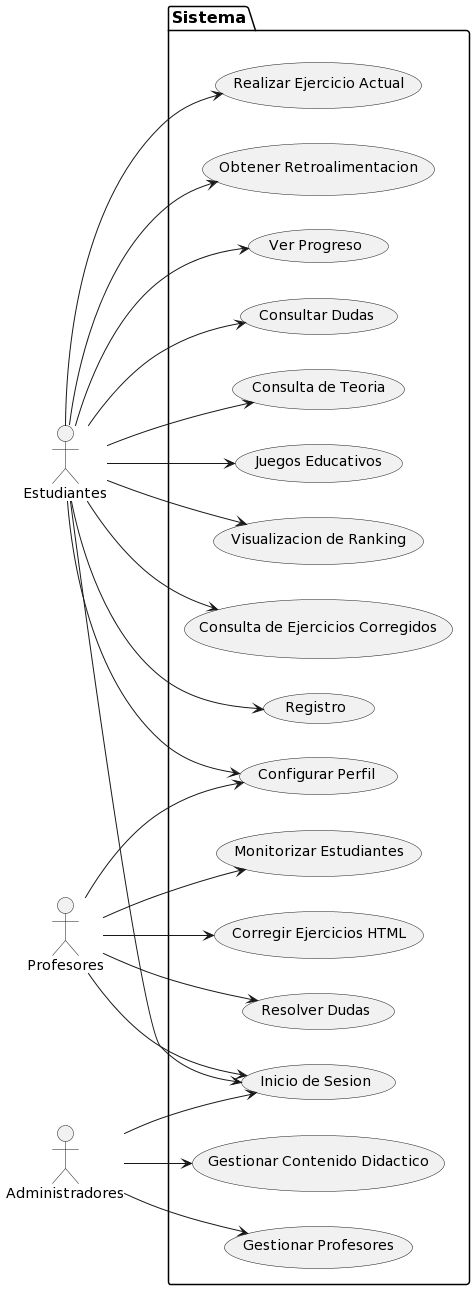
\includegraphics[width=0.4\textwidth]{imagenes/modelo.png}
    \caption{Diagrama de Caso de Uso del sistema}
    \label{fig:caso_uso}
\end{figure}

\subsection{Escenarios de Uso Detallados} \label{sec:comportamiento}

En esta subsección, se realiza un análisis de los escenarios de uso que involucran a los diferentes tipos de usuarios de la plataforma. Para cada escenario, se presentarán tablas detalladas que ofrecen una comprensión clara de cómo los usuarios interactúan con el sistema. Estos escenarios son esenciales para entender las funcionalidades y la respuesta del sistema ante las necesidades de los usuarios.

Los elementos que compondrán cada tabla de escenarios de uso son los siguientes, siguiendo las pautas recomendadas por expertos en usabilidad:

\begin{itemize}
    \item \textbf{ID}: Código de identificación único para cada escenario de uso.
    \item \textbf{Nombre}: Título descriptivo para el escenario de uso.
    \item \textbf{Actor}: Definición de los usuarios implicados en la acción.
    \item \textbf{Descripción}: Breve explicación del escenario de uso. 
    \item \textbf{Precondiciones}: Condiciones previas necesarias para que se inicie el escenario
    \item \textbf{Postcondición}: Estado o resultado alcanzado tras completar el escenario.
    \item \textbf{Flujo}:Detalle de todos los pasos del escenario, incluyendo flujos básicos y alternativos.
\end{itemize}

Los escenarios se centran en aspectos cruciales de la plataforma, enfatizando aquellos factores más relevantes y únicos. Se ha decidido omitir escenarios de uso comunes y autoexplicativos, como el inicio de sesión, registro o cierre de sesión, para centrarse en aquellos que aportan una mayor comprensión de las funcionalidades específicas y la interacción del usuario con la plataforma.

\begin{table}[H]
    \centering
    \begin{tabularx}{\textwidth}{|l|X|}
    \hline
    ID & EU-1 \\
    \hline
    Nombre & Realización de un ejercicio \\
    \hline
    Actor & Estudiante \\
    \hline
    Descripción & El estudiante resuelve un ejercicio de programación. \\
    \hline
    Precondiciones & EEstudiante ha iniciado sesión y ha seleccionado un módulo pendiente. \\
    \hline
    Postcondición & El ejercicio se marca como completado y el estudiante recibe retroalimentación. \\
    \hline
    Flujo & 
    1. El estudiante accede al módulo pendiente. \\
    & 2. Se abre un ejercicio para realizar. \\
    & 3. Resuelve el ejercicio dentro del tiempo establecido. \\
    & 4. Envía la solución para su evaluación. \\
    & 5. Recibe retroalimentación y puntuación. \\
    \hline
    \end{tabularx}
    \caption{EU-1: Realización de un ejercicio}
\end{table}

\begin{table}[H]
    \centering
    \begin{tabularx}{\textwidth}{|l|X|}
    \hline
    ID & EU-2 \\
    \hline
    Nombre & Tiempo superado en un ejercicio \\
    \hline
    Actor & Estudiante \\
    \hline
    Descripción & El estudiante no logra completar un ejercicio de programación dentro del tiempo límite. \\
    \hline
    Precondiciones & Estudiante ha iniciado sesión y está resolviendo un ejercicio. \\
    \hline
    Postcondición & El ejercicio se marca como erróneo y se le muestra un nuevo ejercicio. \\
    \hline
    Flujo & 
    1. Estudiante trabaja en un ejercicio. \\
    & 2. No completa el ejercicio en el tiempo límite. \\
    & 3. El sistema marca el ejercicio como fallido. \\
    & 4. Se presenta automáticamente un nuevo ejercicio al estudiante. \\
    \hline
    \end{tabularx}
    \caption{EU-2: Tiempo superado en un ejercicio}
\end{table}

\begin{table}[H]
    \centering
    \begin{tabularx}{\textwidth}{|l|X|}
    \hline
    ID & EU-3\\
    \hline
    Nombre & Corrección de ejercicios por parte del profesor \\
    \hline
    Actor & Profesor \\
    \hline
    Descripción & El profesor corrige manualmente ejercicios HTML debido a su complejidad. \\
    \hline
    Precondiciones & Profesor ha iniciado sesión y tiene ejercicios HTML pendientes de corrección. \\
    \hline
    Postcondición & Ejercicio corregido y retroalimentación enviada al estudiante. \\
    \hline
    Flujo & 
    1. Profesor revisa la lista de ejercicios HTML pendientes. \\
    & 2. Selecciona un ejercicio para corregir. \\
    & 3. Evalúa el ejercicio y redacta comentarios de retroalimentación. \\
    & 4. Marca el ejercicio como corregido y envía la retroalimentación. \\
    \hline
    \end{tabularx}
    \caption{EU-3: Corrección de ejercicios por parte del profesor}
\end{table}

\begin{table}[H]
    \centering
    \begin{tabularx}{\textwidth}{|l|X|}
    \hline
    ID & EU-4 \\
    \hline
    Nombre & Administrador gestionando contenido didáctico \\
    \hline
    Actor & Administrador \\
    \hline
    Descripción & El administrador añade, consulta edita o elimina contenido educativo en la plataforma. \\
    \hline
    Precondiciones & Administrador ha iniciado sesión. \\
    \hline
    Postcondición & Contenido educativo actualizado en la plataforma. \\
    \hline
    Flujo & 
    1. Administrador accede al módulo de gestión de contenido. \\
    & 2. Elige entre añadir, editar o eliminar contenido. \\
    & 3. Realiza la acción seleccionada y revisa los cambios. \\
    & 4. Confirma y actualiza el contenido en la plataforma. \\
    \hline
    \end{tabularx}
    \caption{EU-4: Gestión del contenido didáctico}
\end{table}

\begin{table}[H]
    \centering
    \begin{tabularx}{\textwidth}{|l|X|}
    \hline
    ID & EU-5 \\
    \hline
    Nombre & Resolución de dudas \\
    \hline
    Actor & Estudiante, Profesor \\
    \hline
    Descripción & El estudiante plantea una duda y el profesor la resuelve. \\
    \hline
    Precondiciones & Estudiante y profesor han iniciado sesión. \\
    \hline
    Postcondición & Duda resuelta. \\
    \hline
    Flujo & 
    1. Estudiante envía una pregunta en la sección de dudas. \\
    & 2. Profesor revisa las dudas pendientes en su panel. \\
    & 3. Selecciona y responde la duda del estudiante. \\
    & 4. Estudiante recibe la respuesta y notificación de duda resuelta. \\
    \hline
    \end{tabularx}
    \caption{EU-5: Resolución de dudas}
\end{table}

\begin{table}[H]
    \centering
    \begin{tabularx}{\textwidth}{|l|X|}
    \hline
    ID & EU-6 \\
    \hline
    Nombre & Seguimiento del Progreso del Estudiante \\
    \hline
    Actor & Profesor \\
    \hline
    Descripción & El profesor revisa y hace seguimiento del progreso de los estudiantes en sus ejercicios y módulos. \\
    \hline
    Precondiciones & Profesor ha iniciado sesión. \\
    \hline
    Postcondición & Comprensión actualizada del progreso del estudiante. \\
    \hline
    Flujo & 
    1. Profesor accede al panel de seguimiento. \\
    & 2. Selecciona un estudiante para revisar su progreso. \\
    & 3. Analiza el rendimiento del estudiante en ejercicios y módulos. \\
    \hline
    \end{tabularx}
    \caption{EU-6: Seguimiento del Progreso del Estudiante}
\end{table}

\begin{table}[H]
    \centering
    \begin{tabularx}{\textwidth}{|l|X|}
    \hline
    ID & EU-7 \\
    \hline
    Nombre &  Gestión de Usuarios \\
    \hline
    Actor & Administrador \\
    \hline
    Descripción & El administrador gestiona las cuentas de usuario, incluyendo la creación, consulta, modificación y eliminación de cuentas de estudiantes y profesores. \\
    \hline
    Precondiciones & Administrador ha iniciado sesión. \\
    \hline
    Postcondición &  Las cuentas de usuario son actualizadas según las acciones realizadas. \\
    \hline
    Flujo & 
    1. Administrador accede al panel de gestión de usuarios. \\
    & 2. Elige entre crear, modificar o eliminar cuentas. \\
    & 3. Realiza la acción seleccionada y revisa los cambios. \\
    & 4. Guarda los cambios y actualiza el registro de usuarios. \\
    \hline
    \end{tabularx}
    \caption{EU-7: Gestión de usuarios}
\end{table}

\subsection{Restricciones y Reglas de Negocio}

Esta subsección detalla las pautas operativas y limitaciones que rigen la interacción de los usuarios con el sistema. Se establecen restricciones específicas para cada tipo de usuario y se definen reglas clave que garantizan un entorno seguro y eficiente, delineando así las condiciones bajo las cuales opera la plataforma educativa.

\paragraph{Restricciones de Acceso}
\begin{itemize}
\item \textbf{Estudiantes}: Su acceso se limita a los módulos y ejercicios específicamente asignados por la plataforma, garantizando un aprendizaje estructurado.
\item \textbf{Profesores}: Capacidad de acceder a la corrección de ejercicios HTML, al panel de dudas y a consultar el progreso de los estudiantes, pero sin permisos para modificar el contenido didáctico.
\item \textbf{Administradores}: Poseen control total sobre la gestión del contenido y las cuentas de los profesores, asegurando la calidad y la actualización constante de la plataforma.
\end{itemize}

\paragraph{Reglas de Validación}
\begin{itemize}
\item Los ejercicios deben completarse dentro de un tiempo límite establecido; si se excede, se considerarán fallidos.
\item La puntuación se asigna en base a la corrección y calidad del código entregado.
\item Los ejercicios HTML requieren una validación manual específica por parte de los profesores.
\end{itemize}

\paragraph{Reglas de Negocio Adicionales}
\begin{itemize}
\item Si un estudiante falla en un ejercicio, se le asigna un nuevo problema como medida para prevenir la desmotivación o frustración.
\item Los profesores tienen la capacidad de identificar a estudiantes con bajo rendimiento o inactividad prolongada, y deben enviar correos motivacionales para apoyarlos.
\item La autorización para añadir o eliminar cuentas de profesores está reservada exclusivamente a los administradores.
\item Proceso de registro controlado para añadir estudiantes, sin posibilidad de inclusión directa por parte de administradores o profesores.
\item Prohibición de borrado de datos de estudiantes, garantizando la integridad y privacidad de la información.
\end{itemize}

\subsection{Seguridad y Acceso}

Para garantizar la integridad de la plataforma, se deben abordar aspectos de seguridad y acceso.

\paragraph{Autenticación} La plataforma adopta un sistema de autenticación, concretamente se logra mediante el uso de correo electrónico y contraseña. 

\paragraph{Autorización} Diferentes roles de usuario, como estudiantes, profesores y administradores, tienen niveles de acceso específicos. Por ejemplo, mientras que los profesores pueden corregir ejercicios y resolver dudas, no tienen autorización para modificar el contenido educativo.

\paragraph{Seguridad de Datos} La protección de los datos es una alta prioridad. Las contraseñas se almacenan de forma segura, empleando técnicas modernas de hash y salting. 

\paragraph{Monitorización y Auditoría} Se lleva a cabo una monitorización constante de todas las actividades significativas dentro de la plataforma. Esto no solo permite a los administradores realizar seguimientos detallados, sino que también facilita la identificación y respuesta rápida ante cualquier actividad inusual o sospechosa, mejorando así la seguridad y la eficiencia del sistema.

\section{Modelado de Datos y Diagrama Entidad-Relación} \label{sec:er}

El modelado de datos es fundamental para entender cómo se van a estructurar y relacionar las diferentes entidades dentro de la base de datos. 

En este proyecto, entidades como Estudiantes, Módulos, Requisitos, Ejercicios, Teorías, Preguntas, Juegos interactúan entre sí, formando el núcleo de la lógica operativa y las funcionalidades del sistema. Además, se introducen entidades adicionales que refuerzan y detallan aún más este modelo. El Diagrama Entidad-Relación (ER), presentado en la Figura \ref{fig:er}, proporciona una representación visual detallada de estas interacciones.

En el diagrama, se destacan las siguientes entidades clave y sus roles específicos en el sistema:

\begin{itemize}
    \item \textbf{Users}: Incluyen a estudiantes, profesores y administradores, cada uno interactuando con el sistema de manera única.
    \item \textbf{Questions}: Representan consultas o dudas planteadas por los estudiantes, vinculadas a ejercicios o teorías específicas.
    \item \textbf{Exercises}: Tareas individuales que están integradas en un requisito de un módulo concreto, representando desafíos prácticos para los estudiantes.
    \item \textbf{Theory}: Material didáctico vinculado a cada requisito de un módulo, proporcionando el marco teórico necesario.
    \item \textbf{Modules}: Agrupan ejercicios y teoría, estructurando el contenido educativo en torno a temas específicos de programación.
    \item  \textbf{Requirements}: Establecen los objetivos educativos para los módulos, siendo cada requisito un elemento concreto de la programación que se quiere enseñar.
    \item \textbf{Games}: Actividades de gamificación diseñadas para mejorar la experiencia de aprendizaje y motivar a los estudiantes.
    \item \textbf{Payments}: Gestionan las transacciones en las que los estudiantes usan puntos acumulados para adquirir juegos.
    \item \textbf{Notifications}: Gestiona las alertas y mensajes que los estudiantes reciben, vital para la comunicación y el seguimiento del estudiante.
    \item \textbf{StudentProgress y StudentActivity}: Registra el avance y la actividad de cada estudiante en el sistema, lo que permite un seguimiento personalizable y adaptable de su aprendizaje.
    \item \textbf{TheoryRequirements y ExerciseRequirements}: Define los requisitos previos para acceder a ciertos ejercicios y materiales teóricos, asegurando una progresión lógica en el aprendizaje.
    \item \textbf{ExtraExercises}: Si es pertinente, se almacena por estudiante unos ejercicios concretos que debe realizar.
    \item \textbf{StudentModules}: Relacionan a los estudiantes con los módulos específicos donde se encuentran. 
    \item \textbf{ModuleRequirementsOrder}: Establecen un orden lógico para los módulos y sus requisitos, garantizando una estructura educativa coherente.
    \item \textbf{UserRequirementsCompleted}: Registran los requisitos completados por los usuarios.
\end{itemize}

Las relaciones entre estas entidades son esenciales para el funcionamiento eficaz del sistema. Por ejemplo, los módulos están formados por requisitos que contienen ejercicios y teoría, formando un plan de estudios coherente. Los juegos añaden un elemento interactivo y lúdico, mientras que los registros de pagos controlan el uso de puntos para el acceso a estos. Las preguntas, por otro lado, facilitan la interacción directa entre estudiantes y profesores, enriqueciendo el proceso de aprendizaje.

\begin{figure}[H]
    \centering
    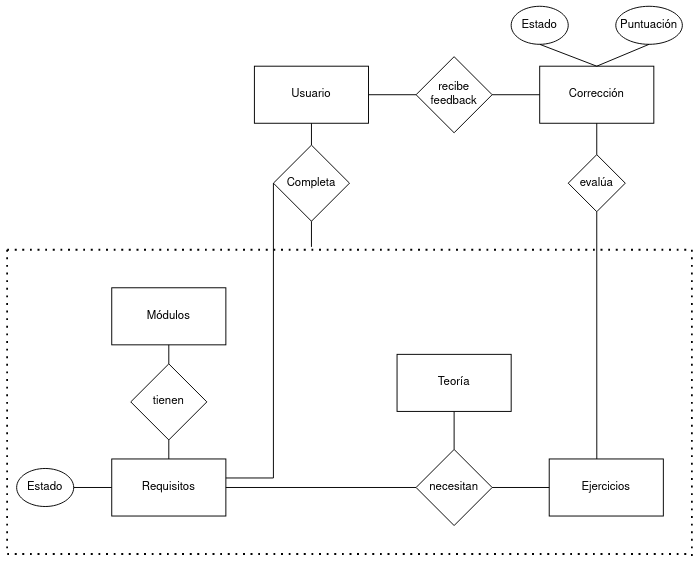
\includegraphics[width=0.8\textwidth]{imagenes/Entidad-Relacion.png}
    \caption{Diagrama Entidad-Relación del sistema}
    \label{fig:er}
\end{figure}



    \chapter{Requisitos} \label{chap:requisitos}

Basado en el análisis presentado anteriormente, este capítulo se dedica a perfilar los requisitos de la plataforma. La evaluación previa ha establecido un fundamento detallar dichos requisitos. Estos serán el eje que dirigirá el proceso de desarrollo, con el propósito de garantizar que la plataforma resultante satisfaga plenamente las expectativas y requisitos de los usuarios finales.

\section{Requisitos Funcionales}

Con tal de garantizar la funcionalidad del programa y la realización de los objetivos establecidos, es esencial tener una buena definición de los requisitos funcionales. Para facilitar su comprensión, presentaremos estos requisitos en tablas, siguiendo las convenciones de la ingeniería de requisitos y desarrollo de software. La organización de los contenidos es la siguiente:

\begin{itemize}
    \item \textbf{ID}: Identificador único para cada requisito. Esencial para una fácil referencia y seguimiento.
    \item \textbf{Nombre}: Nombre del requisito.
    \item \textbf{Descripción}: Explicación del propósito y alcance del requisito.
    \item \textbf{Prioridad}: La importancia del requisito en relación con el sistema. Las categorías posibles son alta, media o baja. Siendo crucial abordar primero los requisitos de alta prioridad, mientras que los de baja prioridad se harán al final.
    \item \textbf{Estado}: Refleja la situación actual del requisito, pudiendo estar \textit{en desarrollo}, \textit{completado}, \textit{en revisión} o \textit{rechazado}.
\end{itemize}


\subsection{Generales}

\begin{table}[H]
    \centering
    \begin{tabular}{|l|p{9.5cm}|}
        \hline
        \textbf{ID} & RF-01 \\
        \hline
        \textbf{Nombre} & Inicio de sesión \\
        \hline
        \textbf{Descripción} & Los usuarios registrados deben poder acceder a la plataforma introduciendo su nombre de usuario y contraseña. El sistema debe garantizar la confidencialidad y autenticidad de esta operación, asegurando que las contraseñas se gestionan y almacenan de manera segura. \\
        \hline
        \textbf{Prioridad} & Alta \\
        \hline
        \textbf{Estado} & Completado \\
        \hline
    \end{tabular}
    \caption{Requisito funcional RF-01: Inicio de sesión.}
    \label{table:req-RF001}
\end{table}

\begin{table}[H]
    \centering
    \begin{tabular}{|l|p{9.5cm}|}
        \hline
        \textbf{ID} & RF-02 \\
        \hline
        \textbf{Nombre} & Registro de usuario \\
        \hline
        \textbf{Descripción} & Los nuevos usuarios deben poder registrarse en la plataforma proporcionando información relevante. \\
        \hline
        \textbf{Prioridad} & Alta \\
        \hline
        \textbf{Estado} & Completado \\
        \hline
    \end{tabular}
    \caption{Requisito funcional RF-02: Registro de usuario.}
    \label{table:req-RF002}
\end{table}

\begin{table}[H]
    \centering
    \begin{tabular}{|l|p{9.5cm}|}
        \hline
        \textbf{ID} & RF-03 \\
        \hline
        \textbf{Nombre} & Perfil de usuario \\
        \hline
        \textbf{Descripción} & Cada usuario debe tener un perfil donde pueda visualizar su información personal, y donde poder cambiar ciertos datos.\\
        \hline
        \textbf{Prioridad} & Media \\
        \hline
        \textbf{Estado} & Completado \\
        \hline
    \end{tabular}
    \caption{Requisito funcional RF-03: Perfil de usuario.}
    \label{table:req-RF005}
\end{table}
    

\subsection{Sistema}
        
\begin{table}[H]
    \centering
    \begin{tabular}{|l|p{9.5cm}|}
        \hline
        \textbf{ID} & RF-04 \\
        \hline
        \textbf{Nombre} & Selección de ejercicios por requisitos \\
        \hline
        \textbf{Descripción} & El sistema deberá presentar a los estudiantes ejercicios basados en el requisito que estén estudiando. Una vez completado un ejercicio, el siguiente deberá ser mostrado de forma aleatoria dentro del mismo requisito, hasta que se considere que el estudiante ha asimilado ese requisito. \\
        \hline
        \textbf{Prioridad} & Alta \\
        \hline   
        \textbf{Estado} & Completado \\
        \hline
    \end{tabular}
    \caption{Requisito funcional RF-04: Selección de ejercicios por requisitos.}
    \label{table:req-RF003}
\end{table}

\begin{table}[H]
    \centering
    \begin{tabular}{|l|p{9.5cm}|}
        \hline
        \textbf{ID} & RF-05 \\
        \hline
        \textbf{Nombre} & Corrección de ejercicios \\
        \hline
        \textbf{Descripción} & Al enviar una solución, el sistema no solo verificará si es correcta, sino que también evaluará la calidad del código en términos de optimización y buenas prácticas de programación. \\
        \hline
        \textbf{Prioridad} & Alta \\
        \hline
        \textbf{Estado} & Completado \\
        \hline
    \end{tabular}
    \caption{Requisito funcional RF-05: Corrección de ejercicios.}
    \label{table:req-RF004}
\end{table}
        
\begin{table}[H]
    \centering
    \begin{tabular}{|l|p{9.5cm}|}
        \hline
        \textbf{ID} & RF-06 \\
        \hline
        \textbf{Nombre} & Compilador integrado \\
        \hline
        \textbf{Descripción} & La plataforma deberá contener con un compilador integrado que permita a los estudiantes probar sus códigos en Java, HTML+CSS+JS, Python y C++. \\
        \hline
        \textbf{Prioridad} & Alta \\
        \hline
        \textbf{Estado} & Completado \\
        \hline
    \end{tabular}
    \caption{Requisito funcional RF-06: Compilador integrado.}
    \label{table:req-RF007}
\end{table}

\begin{table}[H]
    \centering
    \begin{tabular}{|l|p{9.5cm}|}
        \hline
        \textbf{ID} & RF-07 \\
        \hline
        \textbf{Nombre} & Categorización de la teoría \\
        \hline
        \textbf{Descripción} & La teoría se clasificará en función del requisito, facilitando así su visualización dependiendo del punto en que se encuentre el estudiante. \\
        \hline
        \textbf{Prioridad} & Media \\
        \hline
        \textbf{Estado} & Completado \\
        \hline
    \end{tabular}
    \caption{Requisito funcional RF-07: Categorización de la teoría.}
    \label{table:req-RF008}
\end{table}

\begin{table}[H]
    \centering
    \begin{tabular}{|l|p{9.5cm}|}
        \hline
        \textbf{ID} & RF-08 \\
        \hline
        \textbf{Nombre} & Repetición de ejercicios similares tras fallo \\
        \hline
        \textbf{Descripción} & Si un estudiante falla un ejercicio, el sistema deberá presentar otro ejercicio con características similares para que el estudiante pueda intentarlo de nuevo. \\
        \hline
        \textbf{Prioridad} & Alta \\
        \hline
        \textbf{Estado} & Completado \\
        \hline
    \end{tabular}
    \caption{Requisito funcional RF-08: Repetición de ejercicios similares tras fallo.}
    \label{table:req-RF00X}
\end{table}

\begin{table}[H]
    \centering
    \begin{tabular}{|l|p{9.5cm}|}
        \hline
        \textbf{ID} & RF-09 \\
        \hline
        \textbf{Nombre} & Límite de tiempo para completar un ejercicio \\
        \hline
        \textbf{Descripción} & Si el estudiante tarda más de un tiempo predefinido en completar un ejercicio, el sistema lo marcará como erróneo y presentará un nuevo ejercicio. \\
        \hline
        \textbf{Prioridad} & Media \\
        \hline
        \textbf{Estado} & Completado \\
        \hline
    \end{tabular}
    \caption{Requisito funcional RF-09: Límite de tiempo para completar un ejercicio.}
    \label{table:req-RF00Y}
\end{table}

\subsection{Estudiantes}

\begin{table}[H]
    \centering
    \begin{tabular}{|l|p{9.5cm}|}
        \hline
        \textbf{ID} & RF-10 \\
        \hline
        \textbf{Nombre} & Resolución de dudas \\
        \hline
        \textbf{Descripción} & Los estudiantes realizarán preguntas y adjuntar archivos para que el profesor les ayude. \\
        \hline
        \textbf{Prioridad} & Alta \\
        \hline
        \textbf{Estado} & Completado \\
        \hline
    \end{tabular}
    \caption{Requisito funcional RF-10: Resolución de dudas.}
    \label{table:req-RF006}
\end{table}

\begin{table}[H]
    \centering
    \begin{tabular}{|l|p{9.5cm}|}
        \hline
        \textbf{ID} & RF-11 \\
        \hline
        \textbf{Nombre} & Consulta de los rankings \\
        \hline
        \textbf{Descripción} & Los estudiantes podrán consultar un ranking donde vean los \textit{top} 5 estudiantes diarios, semanales y mensuales. \\
        \hline
        \textbf{Prioridad} & Media \\
        \hline
        \textbf{Estado} & Completado \\
        \hline
    \end{tabular}
    \caption{Requisito funcional RF-11: Consulta de los rankings.}
    \label{table:req-RF00Z}
\end{table}

\begin{table}[H]
    \centering
    \begin{tabular}{|l|p{9.5cm}|}
        \hline
        \textbf{ID} & RF-12 \\
        \hline
        \textbf{Nombre} & Juegos en la web \\
        \hline
        \textbf{Descripción} & Por cada módulo que los estudiantes completen, se les desbloqueará un juego como recompensa. \\
        \hline
        \textbf{Prioridad} & Baja \\
        \hline
        \textbf{Estado} & Completado \\
        \hline
    \end{tabular}
    \caption{Requisito funcional RF-12: Juegos en la web.}
    \label{table:req-RF00A}
\end{table}

\begin{table}[H]
    \centering
    \begin{tabular}{|l|p{9.5cm}|}
        \hline
        \textbf{ID} & RF-13 \\
        \hline
        \textbf{Nombre} & Consulta de los ejercicios corregidos \\
        \hline
        \textbf{Descripción} & Los estudiantes podrán consultar los comentarios del profesor sobre los ejercicios que haya corregido. \\
        \hline
        \textbf{Prioridad} & Media \\
        \hline
        \textbf{Estado} & Completado \\
        \hline
    \end{tabular}
    \caption{Requisito funcional RF-13: Consulta de los ejercicios corregidos.}
    \label{table:req-RF00B}
\end{table}

\begin{table}[H]
    \centering
    \begin{tabular}{|l|p{9.5cm}|}
        \hline
        \textbf{ID} & RF-14 \\
        \hline
        \textbf{Nombre} & Sistema de notificación \\
        \hline
        \textbf{Descripción} & Se notificará al estudiante si su ejercicio es correcto o incorrecto cuando lo evalúe el profesor, junto con una retroalimentación del por qué es incorrecto. \\
        \hline
        \textbf{Prioridad} & Alta \\
        \hline
        \textbf{Estado} & Completado \\
        \hline
    \end{tabular}
    \caption{Requisito funcional RF-14: Sistema de notificación.}
    \label{table:req-RF00C}
\end{table}

\begin{table}[H]
    \centering
    \begin{tabular}{|l|p{9.5cm}|}
        \hline
        \textbf{ID} & RF-15 \\
        \hline
        \textbf{Nombre} & Feedback sobre la solución \\
        \hline
        \textbf{Descripción} & Cuando un alumno envíe la solución, se le mostrará un feedback completo sobre ella. \\
        \hline
        \textbf{Prioridad} & Alta \\
        \hline
        \textbf{Estado} & Completado \\
        \hline
    \end{tabular}
    \caption{Requisito funcional RF-15: Feedback sobre la solución.}
    \label{table:req-RF00D}
\end{table}

\begin{table}[H]
    \centering
    \begin{tabular}{|l|p{9.5cm}|}
        \hline
        \textbf{ID} & RF-16 \\
        \hline
        \textbf{Nombre} & Sistema de puntos \\
        \hline
        \textbf{Descripción} & Por cada ejercicio completado, el estudiante obtendrá una cantidad de puntos dependiendo de la calidad de su solución. \\
        \hline
        \textbf{Prioridad} & Baja \\
        \hline
        \textbf{Estado} & Completado \\
        \hline
    \end{tabular}
    \caption{Requisito funcional RF-16: Sistema de puntos.}
    \label{table:req-RF00E}
\end{table}

\subsection{Profesores}

\begin{table}[H]
    \centering
    \begin{tabular}{|l|p{9.5cm}|}
        \hline
        \textbf{ID} & RF-17 \\
        \hline
        \textbf{Nombre} & Lista de usuarios \\
        \hline
        \textbf{Descripción} & El profesor podrá ver una lista de todos los usuarios registrados en la plataforma. \\
        \hline
        \textbf{Prioridad} & Media \\
        \hline
        \textbf{Estado} & Completado \\
        \hline
    \end{tabular}
    \caption{Requisito funcional RF-17: Lista de usuarios.}
    \label{table:req-RF00F}
\end{table}

\begin{table}[H]
    \centering
    \begin{tabular}{|l|p{9.5cm}|}
        \hline
        \textbf{ID} & RF-18 \\
        \hline
        \textbf{Nombre} & Consulta de ejercicios realizados \\
        \hline
        \textbf{Descripción} & El profesor podrá consultar los ejercicios realizados por los estudiantes, junto con su estado, \\
        \hline
        \textbf{Prioridad} & Media \\
        \hline
        \textbf{Estado} & Completado \\
        \hline
    \end{tabular}
    \caption{Requisito funcional RF-18: Consulta de ejercicios realizados.}
    \label{table:req-RF00G}
\end{table}


\begin{table}[H]
    \centering
    \begin{tabular}{|l|p{9.5cm}|}
        \hline
        \textbf{ID} & RF-19 \\
        \hline
        \textbf{Nombre} & Panel de resolución de preguntas \\
        \hline
        \textbf{Descripción} & El profesor tendrá un panel donde podrá responder las preguntas realizadas por los estudiantes. \\
        \hline
        \textbf{Prioridad} & Alta \\
        \hline
        \textbf{Estado} & Completado \\
        \hline
    \end{tabular}
    \caption{Requisito funcional RF-19: Panel de resolución de preguntas.}
    \label{table:req-RF00H}
\end{table}

\begin{table}[H]
    \centering
    \begin{tabular}{|l|p{9.5cm}|}
        \hline
        \textbf{ID} & RF-20 \\
        \hline
        \textbf{Nombre} & Lista de estudiantes inactivos \\
        \hline
        \textbf{Descripción} & El profesor podrá consultar en una lista los estudiantes que llevan más de una semana sin conectarse, incluyendo sus correos electrónicos para un posible seguimiento. \\
        \hline
        \textbf{Prioridad} & Media \\
        \hline
        \textbf{Estado} & Completado \\
        \hline
    \end{tabular}
    \caption{Requisito funcional RF-20: Lista de estudiantes inactivos.}
    \label{table:req-RF00I}
\end{table}

\begin{table}[H]
    \centering
    \begin{tabular}{|l|p{9.5cm}|}
        \hline
        \textbf{ID} & RF-21\\
        \hline
        \textbf{Nombre} & Tiempo de resolución de ejercicios \\
        \hline
        \textbf{Descripción} & Habrá una lista de estudiantes que tengan un tiempo de resolución de ejercicios demasiado bajo o alto, con tal de identificar posibles problemas o áreas de mejora. \\
        \hline
        \textbf{Prioridad} & Baja \\
        \hline
        \textbf{Estado} & Completado \\
        \hline
    \end{tabular}
    \caption{Requisito funcional RF-21: Tiempo de resolución de ejercicios.}
    \label{table:req-RF00J}
\end{table}

\begin{table}[H]
    \centering
    \begin{tabular}{|l|p{9.5cm}|}
        \hline
        \textbf{ID} & RF-22 \\
        \hline
        \textbf{Nombre} & Corrección de ejercicios \\
        \hline
        \textbf{Descripción} & El profesor tendrá la capacidad de corregir los ejercicios, relacionados con HTML, enviados por los estudiantes y ser capaz de proporcionar una retroalimentación. \\
        \hline
        \textbf{Prioridad} & Alta \\
        \hline
        \textbf{Estado} & Completado \\
        \hline
    \end{tabular}
    \caption{Requisito funcional RF-22: Corrección de ejercicios.}
    \label{table:req-RF00K}
\end{table}

\begin{table}[H]
    \centering
    \begin{tabular}{|l|p{9.5cm}|}
        \hline
        \textbf{ID} & RF-23 \\
        \hline
        \textbf{Nombre} & Usuarios con múltiples fallos \\
        \hline
        \textbf{Descripción} & Se listarán los usuarios que han fallado más de dos veces un ejercicio específico con tal de poder identificar áreas problemáticas. \\
        \hline
        \textbf{Prioridad} & Baja \\
        \hline
        \textbf{Estado} & Completado \\
        \hline
    \end{tabular}
    \caption{Requisito funcional RF-23: Usuarios con múltiples fallos.}
    \label{table:req-RF00L}
\end{table}

\begin{table}[H]
    \centering
    \begin{tabular}{|l|p{9.5cm}|}
        \hline
        \textbf{ID} & RF-24 \\
        \hline
        \textbf{Nombre} & Ejercicios realizados por día \\
        \hline
        \textbf{Descripción} & Habrá un gráfico donde se podrá consultar el número de ejercicios realizados por día en la plataforma. Con tal de poder evaluar la actividad y el compromiso de los estudiantes. \\
        \hline
        \textbf{Prioridad} & Baja \\
        \hline
        \textbf{Estado} & Completado \\
        \hline
    \end{tabular}
    \caption{Requisito funcional RF-24: Ejercicios realizados por día.}
    \label{table:req-RF00N}
\end{table}

\begin{table}[H]
    \centering
    \begin{tabular}{|l|p{9.5cm}|}
        \hline
        \textbf{ID} & RF-25 \\
        \hline
        \textbf{Nombre} & Usuarios con alta tasa de errores \\
        \hline
        \textbf{Descripción} & Habrá una lista de usuarios con una alta tasa de errores en los ejercicios, con tal de poder ofrecer asistencia adicional. \\
        \hline
        \textbf{Prioridad} & Baja \\
        \hline
        \textbf{Estado} & Completado \\
        \hline
    \end{tabular}
    \caption{Requisito funcional RF-25: Usuarios con alta tasa de errores.}
    \label{table:req-RF00M}
\end{table}

\subsection{Administrador}

\begin{table}[H]
    \centering
    \begin{tabular}{|l|p{9.5cm}|}
        \hline
        \textbf{ID} & RF-26 \\
        \hline
        \textbf{Nombre} & Alta de profesor por administrador \\
        \hline
        \textbf{Descripción} & El administrador tendrá la capacidad de registrar a un profesor mediante el panel de administración. \\
        \hline
        \textbf{Prioridad} & Alta \\
        \hline
        \textbf{Estado} & Completado \\
        \hline
    \end{tabular}
    \caption{Requisito funcional RF-26: Alta de profesor por administrador.}
    \label{table:req-RF0010}
\end{table}
        
\begin{table}[H]
    \centering
    \begin{tabular}{|l|p{9.5cm}|}
        \hline
        \textbf{ID} & RF-27 \\
        \hline
        \textbf{Nombre} & Añadir elementos \\
        \hline
        \textbf{Descripción} & El administrador podrá añadir nuevos módulos, requisitos, profesores, teoría y ejercicios a la plataforma. \\
        \hline
        \textbf{Prioridad} & Alta \\
        \hline
        \textbf{Estado} & Completado \\
        \hline
    \end{tabular}
    \caption{Requisito funcional RF-27: Añadir elementos.}
    \label{table:req-RF00O}
\end{table}

\begin{table}[H]
    \centering
    \begin{tabular}{|l|p{9.5cm}|}
        \hline
        \textbf{ID} & RF-28 \\
        \hline
        \textbf{Nombre} & Consultar elementos \\
        \hline
        \textbf{Descripción} & El administrador podrá consultar los detalles de los módulos, requisitos, profesores, teoría y ejercicios existentes en la plataforma. \\
        \hline
        \textbf{Prioridad} & Alta \\
        \hline
        \textbf{Estado} & Completado \\
        \hline
    \end{tabular}
    \caption{Requisito funcional RF-28: Consultar elementos.}
    \label{table:req-RF00P}
\end{table}

\begin{table}[H]
    \centering
    \begin{tabular}{|l|p{9.5cm}|}
        \hline
        \textbf{ID} & RF-29 \\
        \hline
        \textbf{Nombre} & Editar elementos \\
        \hline
        \textbf{Descripción} & El administrador podrá editar los detalles de los módulos, profesores, teoría y ejercicios, excepto los requisitos que no son editables. \\
        \hline
        \textbf{Prioridad} & Alta \\
        \hline
        \textbf{Estado} & Completado \\
        \hline
    \end{tabular}
    \caption{Requisito funcional RF-29: Editar elementos.}
    \label{table:req-RF00Q}
\end{table}

\begin{table}[H]
    \centering
    \begin{tabular}{|l|p{9.5cm}|}
        \hline
        \textbf{ID} & RF-30 \\
        \hline
        \textbf{Nombre} & Eliminar elementos \\
        \hline
        \textbf{Descripción} & El administrador podrá eliminar módulos, requisitos, profesores, teoría y ejercicios de la plataforma. \\
        \hline
        \textbf{Prioridad} & Alta \\
        \hline
        \textbf{Estado} & Completado \\
        \hline
    \end{tabular}
    \caption{Requisito funcional RF-30: Eliminar elementos.}
    \label{table:req-RF00R}
\end{table}

\begin{table}[H]
    \centering
    \begin{tabular}{|l|p{9.5cm}|}
        \hline
        \textbf{ID} & RF-31 \\
        \hline
        \textbf{Nombre} & Orden global \\
        \hline
        \textbf{Descripción} & El administrador podrá crear y consultar un orden global que especifica el camino que debe seguir el estudiante en la plataforma, siendo una secuencia de módulos y requisitos. \\
        \hline
        \textbf{Prioridad} & Alta \\
        \hline
        \textbf{Estado} & Completado \\
        \hline
    \end{tabular}
    \caption{Requisito funcional RF-31: Orden global.}
    \label{table:req-RF00S}
\end{table}


\section{Requisitos No Funcionales}

Con tal de asegurar la calidad global del sistema, deberemos tener en cuenta los requisitos no funcionales. Por ello, se van a detallar estos requisitos de manera estructurada siguiendo el mismo formato que con los requisitos funcionales.

\begin{table}[H]
    \centering
    \begin{tabular}{|l|p{9.5cm}|}
        \hline
        \textbf{ID} & RNF-01 \\
        \hline
        \textbf{Nombre} & Usabilidad \\
        \hline
        \textbf{Descripción} & El sistema deberá ser intuitivo y fácil de usar para los diferentes tipos de usuarios. \\
        \hline
        \textbf{Prioridad} & Alta \\
        \hline
        \textbf{Estado} & Completado \\
        \hline
    \end{tabular}
    \caption{Requisito no funcional RNF-01: Usabilidad.}
    \label{table:req-RNF31}
\end{table}

\begin{table}[H]
    \centering
    \begin{tabular}{|l|p{9.5cm}|}
        \hline
        \textbf{ID} & RNF-02 \\
        \hline
        \textbf{Nombre} & Rendimiento \\
        \hline
        \textbf{Descripción} & El sistema deberá ser capaz de manejar una cantidad promedio de usuarios. \\
        \hline
        \textbf{Prioridad} & Media \\
        \hline
        \textbf{Estado} & Completado \\
        \hline
    \end{tabular}
    \caption{Requisito no funcional RNF-02: Rendimiento.}
    \label{table:req-RNF32}
\end{table}

\begin{table}[H]
    \centering
    \begin{tabular}{|l|p{9.5cm}|}
        \hline
        \textbf{ID} & RNF-03 \\
        \hline
        \textbf{Nombre} & Seguridad \\
        \hline
        \textbf{Descripción} & Todos los datos sensibles, como contraseñas, deben estar encriptados. \\
        \hline
        \textbf{Prioridad} & Alta \\
        \hline
        \textbf{Estado} & Completado \\
        \hline
    \end{tabular}
    \caption{Requisito no funcional RNF-03: Seguridad.}
    \label{table:req-RNF33}
\end{table}

\begin{table}[H]
    \centering
    \begin{tabular}{|l|p{9.5cm}|}
        \hline
        \textbf{ID} & RNF-04 \\
        \hline
        \textbf{Nombre} & Compatibilidad \\
        \hline
        \textbf{Descripción} & El sistema debe ser compatible con los navegadores web más comunes, incluidos Chrome, Firefox y Safari. \\
        \hline
        \textbf{Prioridad} & Alta \\
        \hline
        \textbf{Estado} & Completado \\
        \hline
    \end{tabular}
    \caption{Requisito no funcional RNF-04: Compatibilidad.}
    \label{table:req-RNF35}
\end{table}

\begin{table}[H]
    \centering
    \begin{tabular}{|l|p{9.5cm}|}
        \hline
        \textbf{ID} & RNF-05 \\
        \hline
        \textbf{Nombre} & Escalabilidad \\
        \hline
        \textbf{Descripción} & El sistema deberá ser escalable para permitir la adición de más módulos, ejercicios y usuarios en el futuro. \\
        \hline
        \textbf{Prioridad} & Alta \\
        \hline
        \textbf{Estado} & Completado \\
        \hline
    \end{tabular}
    \caption{Requisito no funcional RNF-05: Escalabilidad.}
    \label{table:req-RNF36}
\end{table}

\begin{table}[H]
    \centering
    \begin{tabular}{|l|p{9.5cm}|}
        \hline
        \textbf{ID} & RNF-06 \\
        \hline
        \textbf{Nombre} & Disponibilidad \\
        \hline
        \textbf{Descripción} & La página web debe estar disponible el 99\% del tiempo, excluyendo el tiempo de mantenimiento programado. \\
        \hline
        \textbf{Prioridad} & Media \\
        \hline
        \textbf{Estado} & Completado \\
        \hline
    \end{tabular}
    \caption{Requisito no funcional RNF-06: Disponibilidad.}
    \label{table:req-RNF37}
\end{table}

\begin{table}[H]
    \centering
    \begin{tabular}{|l|p{9.5cm}|}
        \hline
        \textbf{ID} & RNF-07 \\
        \hline
        \textbf{Nombre} & Tiempo de Respuesta \\
        \hline
        \textbf{Descripción} & El tiempo de carga de las páginas no debe superar los 5 segundos. \\
        \hline
        \textbf{Prioridad} & Media \\
        \hline
        \textbf{Estado} & Completado \\
        \hline
    \end{tabular}
    \caption{Requisito no funcional RNF-07: Tiempo de Respuesta.}
    \label{table:req-RNF38}
\end{table}


\begin{table}[H]
    \centering
    \begin{tabular}{|l|p{9.5cm}|}
        \hline
        \textbf{ID} & RNF-08 \\
        \hline
        \textbf{Nombre} & Mantenimiento \\
        \hline
        \textbf{Descripción} & Se deberá tener una arquitectura bien estructurada que facilite poder añadir nuevas funcionalidades. Además, de poder corregir errores sin afectar al funcionamiento de todo el sistema  \\
        \hline
        \textbf{Prioridad} & Alta \\
        \hline
        \textbf{Estado} & Completado \\
        \hline
    \end{tabular}
    \caption{Requisito no funcional RNF-08: Mantenimiento.}
    \label{table:req-RNF39}
\end{table}

\section{Requisitos de Información}

Dentro del marco de requisitos esenciales para el desarrollo de la plataforma, los requisitos de información también tienen su papel. Estos requisitos deben definir cómo debe ser recolectada, almacenada, procesada y protegida la información dentro del sistema. 

La organización de los contenidos de los requisitos de información es la siguiente:

\begin{itemize}
    \item \textbf{ID}: Identificador único para cada requisito. Esencial para una fácil referencia y seguimiento durante todo el ciclo de vida del desarrollo del software.
    \item \textbf{Nombre}: El nombre del requisito, que se corresponde directamente con cada entidad de la base de datos para facilitar la correlación.
    \item \textbf{Descripción}: Una explicación del tipo de datos dentro del sistema.
    \item \textbf{Contenido}: Detalles específicos sobre la información que se almacena, incluyendo formatos, estructuras y cualquier restricción relevante.
\end{itemize}

\begin{table}[H]
    \centering
    \begin{tabular}{|l|p{9.5cm}|}
        \hline
        \textbf{ID} & RI-01 \\
        \hline
        \textbf{Nombre} & Usuario \\
        \hline
        \textbf{Descripción} & Datos esenciales de los usuarios para permitir el acceso y la interacción con el sistema. \\
        \hline
        \textbf{Contenido} & Información básica del usuario como nombre, apellidos, fecha de nacimiento, contacto y credenciales de acceso. También se incluye información para el seguimiento del progreso educativo y la interacción con el sistema. \\
        \hline
    \end{tabular}
    \caption{Requisito de información RI-01: Usuario.}
    \label{table:req-RI01}
\end{table}

\begin{table}[H]
    \centering
    \begin{tabular}{|l|p{9.5cm}|}
        \hline
        \textbf{ID} & RI-02 \\
        \hline
        \textbf{Nombre} & Teoría \\
        \hline
        \textbf{Descripción} &  El sistema almacenará información educativa asociada con los distintos módulos de aprendizaje. \\
        \hline
        \textbf{Contenido} & Incluye el contenido textual de la teoría, identificadores de los módulos relacionados y rutas a recursos gráficos. Se debe mantener la integridad referencial con los módulos del curso.  \\
        \hline
    \end{tabular}
    \caption{Requisito de información RI-02: Teoría.}
    \label{table:req-RI04}
\end{table}

\begin{table}[H]
    \centering
    \begin{tabular}{|l|p{9.5cm}|}
        \hline
        \textbf{ID} & RI-03 \\
        \hline
        \textbf{Nombre} & Ejercicios \\
        \hline
        \textbf{Descripción} & Conjunto de datos que definen los ejercicios prácticos dentro de los módulos del sistema.  \\
        \hline
        \textbf{Contenido} & Información detallada de los ejercicios, como el nombre, contenido descriptivo, soluciones y parámetros de evaluación, así como la identificación de si requieren revisión manual o son ejercicios clave dentro de los módulos.  \\
        \hline
    \end{tabular}
    \caption{Requisito de información RI-03: Ejercicios.}
    \label{table:req-RI05}
\end{table}

\begin{table}[H]
    \centering
    \begin{tabular}{|l|p{9.5cm}|}
        \hline
        \textbf{ID} & RI-04 \\
        \hline
        \textbf{Nombre} & Juegos \\
        \hline
        \textbf{Descripción} & Datos relacionados con los juegos disponibles en la plataforma. \\
        \hline
        \textbf{Contenido} & Título de cada juego y su costo asociado, que puede utilizarse para transacciones o recompensas dentro del sistema educativo de la plataforma. \\
        \hline
    \end{tabular}
    \caption{Requisito de información RI-04: Juegos.}
    \label{table:req-RI06}
\end{table}

\begin{table}[H]
    \centering
    \begin{tabular}{|l|p{9.5cm}|}
        \hline
        \textbf{ID} & RI-05 \\
        \hline
        \textbf{Nombre} & Progreso del estudiante \\
        \hline
        \textbf{Descripción} & Registro detallado del avance de cada estudiante en los ejercicios y módulos del curso. \\
        \hline
        \textbf{Contenido} & Información de progreso que incluye el estado del ejercicio (completado, en progreso, etc.), calificaciones, fechas relevantes, código de solución proporcionado por el estudiante, y cualquier comentario del instructor o puntuación de evaluación automática. \\
        \hline
    \end{tabular}
    \caption{Requisito de información RI-05: Progreso del estudiante.}
    \label{table:req-RI07}
\end{table}

\begin{table}[H]
    \centering
    \begin{tabular}{|l|p{9.5cm}|}
        \hline
        \textbf{ID} & RI-06 \\
        \hline
        \textbf{Nombre} & Actividad del estudiante \\
        \hline
        \textbf{Descripción} &  Información que captura las interacciones específicas de los estudiantes con los contenidos del curso. \\
        \hline
        \textbf{Contenido} & Datos sobre las acciones realizadas por el estudiante dentro de la plataforma, incluyendo si han completado o saltado actividades y el tipo de contenido con el que interactuaron, para proporcionar una visión integral de su compromiso con el material del curso. \\
        \hline
    \end{tabular}
    \caption{Requisito de información RI-06: Actividad del estudiante.}
    \label{table:req-RI08}
\end{table}

\begin{table}[H]
    \centering
    \begin{tabular}{|l|p{9.5cm}|}
        \hline
        \textbf{ID} & RI-07 \\
        \hline
        \textbf{Nombre} & Transacciones de Pagos \\
        \hline
        \textbf{Descripción} & Registros de pagos realizados por los usuarios, que detallan la adquisición de los juegos.  \\
        \hline
        \textbf{Contenido} & Detalles de cada transacción, incluyendo el usuario que realiza el pago, el juego o servicio adquirido, la cantidad pagada y la fecha del pago. \\
        \hline
    \end{tabular}
    \caption{Requisito de información RI-07: Transacciones de Pagos.}
    \label{table:req-RI09}
\end{table}

\begin{table}[H]
    \centering
    \begin{tabular}{|l|p{9.5cm}|}
        \hline
        \textbf{ID} & RI-08 \\
        \hline
        \textbf{Nombre} & Notificaciones \\
        \hline
        \textbf{Descripción} & Captura la información de las notificaciones generadas por el sistema o los profesores para los usuarios. \\
        \hline
        \textbf{Contenido} & Datos de las notificaciones como el destinatario, el mensaje específico enviado, la fecha y hora de envío, y un indicador de si la notificación ha sido leída. \\
        \hline
    \end{tabular}
    \caption{Requisito de información RI-08: Notificaciones.}
    \label{table:req-RI10}
\end{table}

\begin{table}[H]
    \centering
    \begin{tabular}{|l|p{9.5cm}|}
        \hline
        \textbf{ID} & RI-09 \\
        \hline
        \textbf{Nombre} & Requisitos \\
        \hline
        \textbf{Descripción} & Información relativa a los requisitos educativos que deben ser cumplidos por los estudiantes en el transcurso de su aprendizaje. Estos requisitos son elementos fundamentales que estructuran los módulos y el contenido del curso.  \\
        \hline
        \textbf{Contenido} & Datos que incluyen un identificador único y el nombre del requisito, que sirve como referencia para la progresión en los módulos y la vinculación con ejercicios y teoría. \\
        \hline
    \end{tabular}
    \caption{Requisito de información RI-09: Requisitos.}
    \label{table:req-RI11}
\end{table}

\begin{table}[H]
    \centering
    \begin{tabular}{|l|p{9.5cm}|}
        \hline
        \textbf{ID} & RI-10 \\
        \hline
        \textbf{Nombre} & \textit{Path} educativo \\
        \hline
        \textbf{Descripción} & Detalles que establecen la secuencia en la que los estudiantes deben cumplir con los requisitos dentro de un módulo específico. Esta secuencia asegura que el proceso de aprendizaje siga una progresión lógica y estructurada.  \\
        \hline
        \textbf{Contenido} & Datos que incluyen el identificador del módulo, el identificador del requisito y la posición que ocupa este requisito en la secuencia de aprendizaje del módulo. \\
        \hline
    \end{tabular}
    \caption{Requisito de información RI-10: \textit{Path} educativo.}
    \label{table:req-RI12}
\end{table}


\begin{table}[H]
    \centering
    \begin{tabular}{|l|p{9.5cm}|}
        \hline
        \textbf{ID} & RI-11 \\
        \hline
        \textbf{Nombre} & Módulo \\
        \hline
        \textbf{Descripción} & Información relacionada con los módulos que componen la estructura curricular de la plataforma. Cada módulo agrupa una serie de requisitos, que a su vez agrupan ejercicios y teoría para facilitar el aprendizaje en temas específicos de la programación. \\
        \hline
        \textbf{Contenido} & Datos que definen cada módulo, incluyendo un identificador único, el nombre del módulo y una descripción que detalla los objetivos y el contenido cubierto.  \\
        \hline
    \end{tabular}
    \caption{Requisito de información RI-11: Módulo.}
    \label{table:req-RI13}
\end{table}

\begin{table}[H]
    \centering
    \begin{tabular}{|l|p{9.5cm}|}
        \hline
        \textbf{ID} & RI-12 \\
        \hline
        \textbf{Nombre} & Preguntas \\
        \hline
        \textbf{Descripción} & Registra las interacciones de los estudiantes en forma de preguntas y respuestas dentro de la plataforma, lo que permite un seguimiento de las dudas y facilita la asistencia por parte del cuerpo docente o de otros estudiantes.  \\
        \hline
        \textbf{Contenido} & Incluye la identificación del estudiante que realiza la pregunta, el texto de la pregunta, la respuesta proporcionada, fechas de realización y respuesta, y cualquier archivo adjunto relevante para la discusión. \\
        \hline
    \end{tabular}
    \caption{Requisito de información RI-12: Preguntas.}
    \label{table:req-RI14}
\end{table}

\begin{table}[H]
    \centering
    \begin{tabular}{|l|p{9.5cm}|}
        \hline
        \textbf{ID} & RI-13 \\
        \hline
        \textbf{Nombre} & Requisitos completados por el usuario \\
        \hline
        \textbf{Descripción} & Contabiliza los requisitos que cada usuario ha completado en los distintos módulos del sistema. Esto permite al sistema y a los instructores monitorear el progreso y asegurar que los estudiantes cumplan con los objetivos educativos establecidos.  \\
        \hline
        \textbf{Contenido} & Incluye el identificador del usuario, el requisito completado, el módulo asociado y la fecha de finalización, permitiendo así una gestión efectiva del avance de cada estudiante. \\
        \hline
    \end{tabular}
    \caption{Requisito de información RI-13: Requisitos completados por el usuario.}
    \label{table:req-RI15}
\end{table}

\begin{table}[H]
    \centering
    \begin{tabular}{|l|p{9.5cm}|}
        \hline
        \textbf{ID} & RI-14 \\
        \hline
        \textbf{Nombre} & Requisitos de teoría \\
        \hline
        \textbf{Descripción} & Asocia los contenidos teóricos con los requisitos educativos específicos, estableciendo las dependencias que los estudiantes deben cumplir para progresar en el aprendizaje teórico del curso.  \\
        \hline
        \textbf{Contenido} & Relaciones entre teorías y requisitos que deben ser completados para acceder a dichos contenidos, asegurando una secuencia lógica de aprendizaje. \\
        \hline
    \end{tabular}
    \caption{Requisito de información RI-14: Requisitos de teoría.}
    \label{table:req-RI16}
\end{table}

\begin{table}[H]
    \centering
    \begin{tabular}{|l|p{9.5cm}|}
        \hline
        \textbf{ID} & RI-15 \\
        \hline
        \textbf{Nombre} & Requisitos de ejercicios\\
        \hline
        \textbf{Descripción} & Define las dependencias entre los ejercicios prácticos y los requisitos educativos, indicando qué conocimientos previos son necesarios para abordar cada ejercicio.  \\
        \hline
        \textbf{Contenido} & Mapeo de los ejercicios con los requisitos correspondientes, lo que permite al sistema validar la preparación del estudiante antes de intentar resolver un ejercicio. \\
        \hline
    \end{tabular}
    \caption{Requisito de información RI-15: Requisitos de los ejercicios.}
    \label{table:req-RI17}
\end{table}

    % Experimentación
    \chapter{Diseño e Implementación} \label{chap:analisisExperimentación}


\section{Diseño Pedagógico}

El diseño pedagógico se centra en el aprendizaje basado en problemas \cite{de2008aprendizaje}. Concretamente, se introduce la teoría relevante, que puede incluir explicaciones de texto, imágenes ilustrativas, y en ocasiones, material en formato de video. Una vez que el usuario ha absorbido el contenido teórico, se le presentan problemas prácticos relacionados para resolver.

Existen dos categorías principales de ejercicios, cada una con un peso distinto en la estructura de aprendizaje:

\begin {enumerate}
\item Ejercicios estándar: Son problemas prácticos que refuerzan la comprensión del usuario sobre el tema.

\item Ejercicios clave (\textit{key\_exercise}): Estos ejercicios desempeñan un papel crucial en la progresión del usuario. Son indicativos de si el usuario ha comprendido los requisitos fundamentales del tema en cuestión. Se deben completar estos ejercicios para avanzar al siguiente tema o módulo. Si el usuario no logra superar estos ejercicios en un primer intento, se le presentan ejercicios adicionales para reforzar su comprensión antes de volver a intentar los ejercicios clave.
\end{enumerate}

La plataforma corrige automáticamente para los módulos de C++, Java y Python, tal como se mencionó con anterioridad. Sin embargo, para el módulo de HTML+CSS+JS, se requiere una revisión manual por parte de un instructor. Esta revisión no solo califica el ejercicio, sino que también proporciona comentarios constructivos para guiar al usuario hacia la solución correcta.

Además de la corrección, la plataforma evalúa la limpieza y estructura del código presentado, ya que es esencial para una buena educación. Por lo tanto, se proporciona una retroalimentación detallada al estudiante no solo sobre la corrección de su respuesta, sino también sobre cómo mejorar y optimizar su código.

Finalmente, la plataforma tiene la capacidad de compilar ejercicios, permitiendo la verificación y corrección del código antes de su envío.

\section{Arquitectura del Sistema}

La interacción del usuario en el Frontend se lleva a cabo utilizando tecnologías estándar como HTML sin emplear \textit{frameworks} adicionales para su desarrollo. Además, la interfaz es \textit{Web Responsive}, lo que garantiza su adaptación a variados dispositivos. Desde el punto de vista de la seguridad, se han implementado medidas como la validación de entradas, previniendo así amenazas como los ataques XSS. Los datos de sesión se conservan en el cliente mediante cookies.

Por otro lado, el Backend se ha desarrollado con Flask. Se encarga de administrar las API RESTful y de establecer una conexión ininterrumpida con la base de datos PostgreSQL. La biblioteca \textit{flask\_login} respalda las funcionalidades de autenticación y autorización, aportando una capa de seguridad adicional. La lógica de negocio del sistema reside principalmente en el Sistema de Tutoría Inteligente (ITS). Este subsistema es el encargado de la elección y evaluación de ejercicios, ofreciendo retroalimentación y monitoreando el avance del estudiante.

En relación con la seguridad del Backend, se han establecido roles y restricciones de acceso coherentes con las reglas de negocio previamente determinadas. Aunque la arquitectura actual no posee herramientas concretas orientadas a la escalabilidad, está concebida para ser resistente y estable.

Es esencial destacar que, la estructura general del sistema sigue el patrón Modelo-Vista-Controlador (MVC). La Vista reside en el Frontend, y el Controlador y Nodelo en el Backend \ref{fig:arqsistema}. Este patrón facilita la distinción entre la lógica de la interfaz de usuario y las operaciones, simplificando su mantenimiento.

\begin{figure}[H]
    \centering
    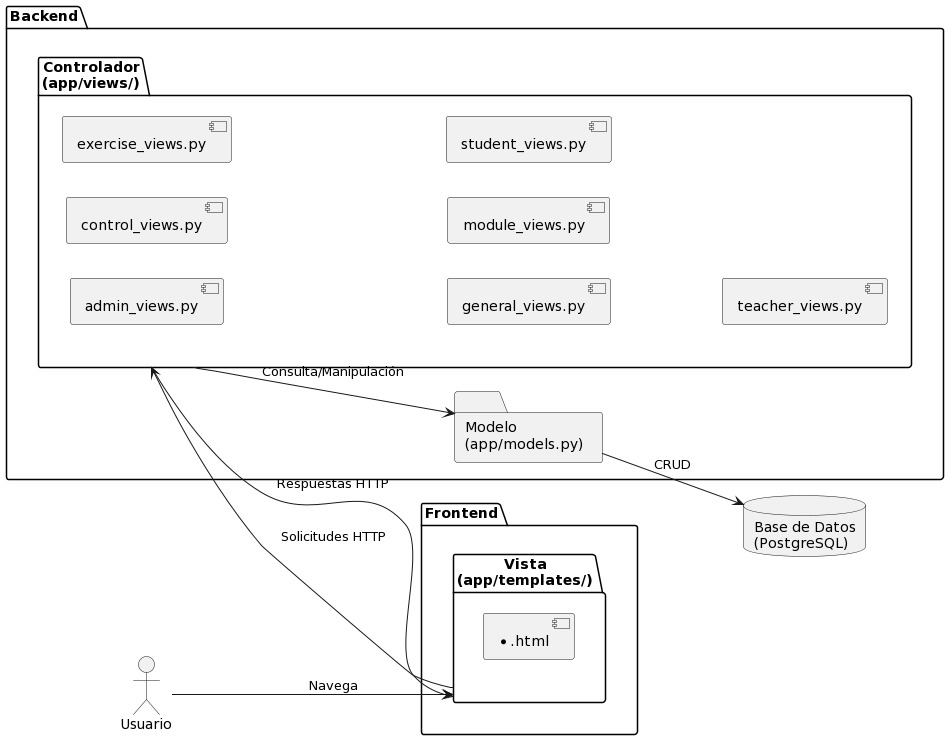
\includegraphics[width=0.55\textwidth]{imagenes/ArquitecturaDeSistema.jpeg}
    
    \caption{Arquitectura de sistema}
    \label{fig:arqsistema}
\end{figure}

\subsection{Diagramas de Arquitectura}
Incluya cualquier diagrama relevante para explicar la arquitectura.

\section{Diseño de Base de Datos}


\newpage

\begin{figure}[H]
    \centering
    \begin{sideways}
        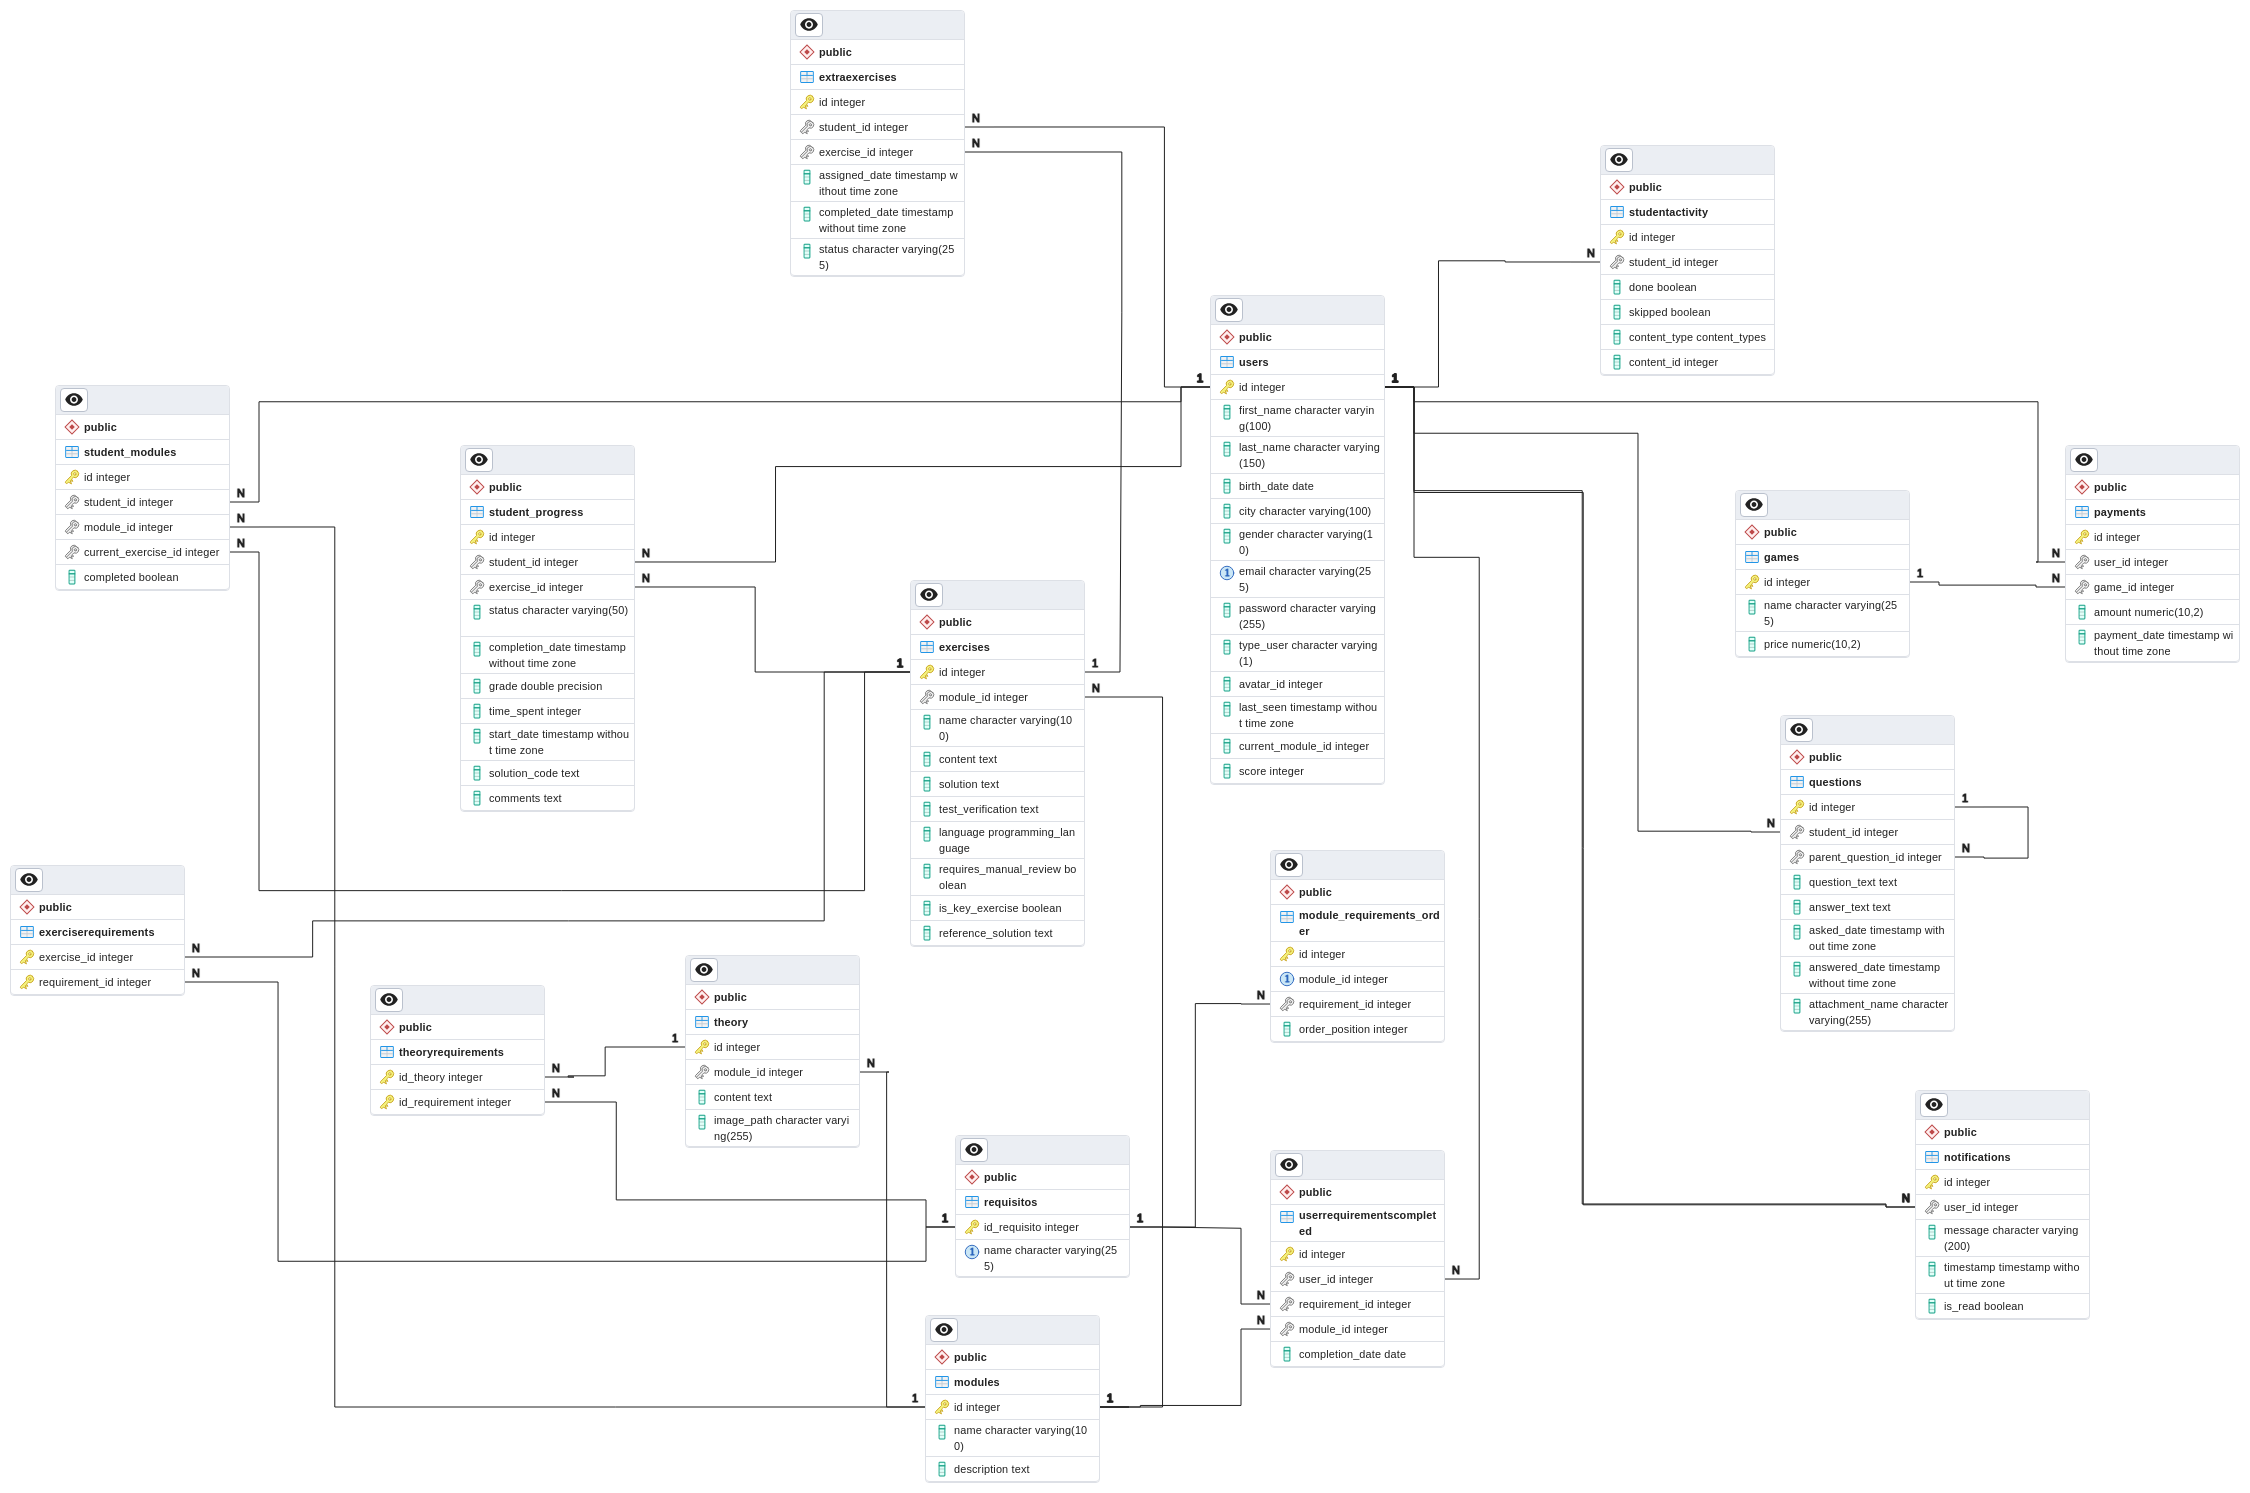
\includegraphics[width=1.8\textwidth]{imagenes/er.png}
    \end{sideways}
    \caption{Diagrama del modelo de datos}
    \label{fig:modeladodedatos}
\end{figure}

\section{Interfaces de Usuario}
\subsection{Mockups o Capturas de Pantalla}
\subsection{Interacción Usuario-Sistema}
Detalles de la interacción del usuario con el sistema.

\section{Implementación de Algoritmos}
\subsection{Algoritmo para la corrección y Evaluación de calidad del código}

El verdadero reto comienza tras la entrega de un ejercicio por parte del estudiante. La lógica de corrección evalúa el código en términos de precisión y calidad. Si un código no alcanza un estándar mínimo, el sistema propone ejercicios adicionales, reforzando así las áreas de mejora del estudiante \ref{fig:correccion}. La justificación detrás de esta lógica se centra en la premisa de que la repetición y el refuerzo son esenciales para consolidar el aprendizaje. Además, al establecer estándares de calidad, se fomentan las buenas prácticas de programación desde las etapas iniciales de formación.

\begin{figure}[H]
    \centering
    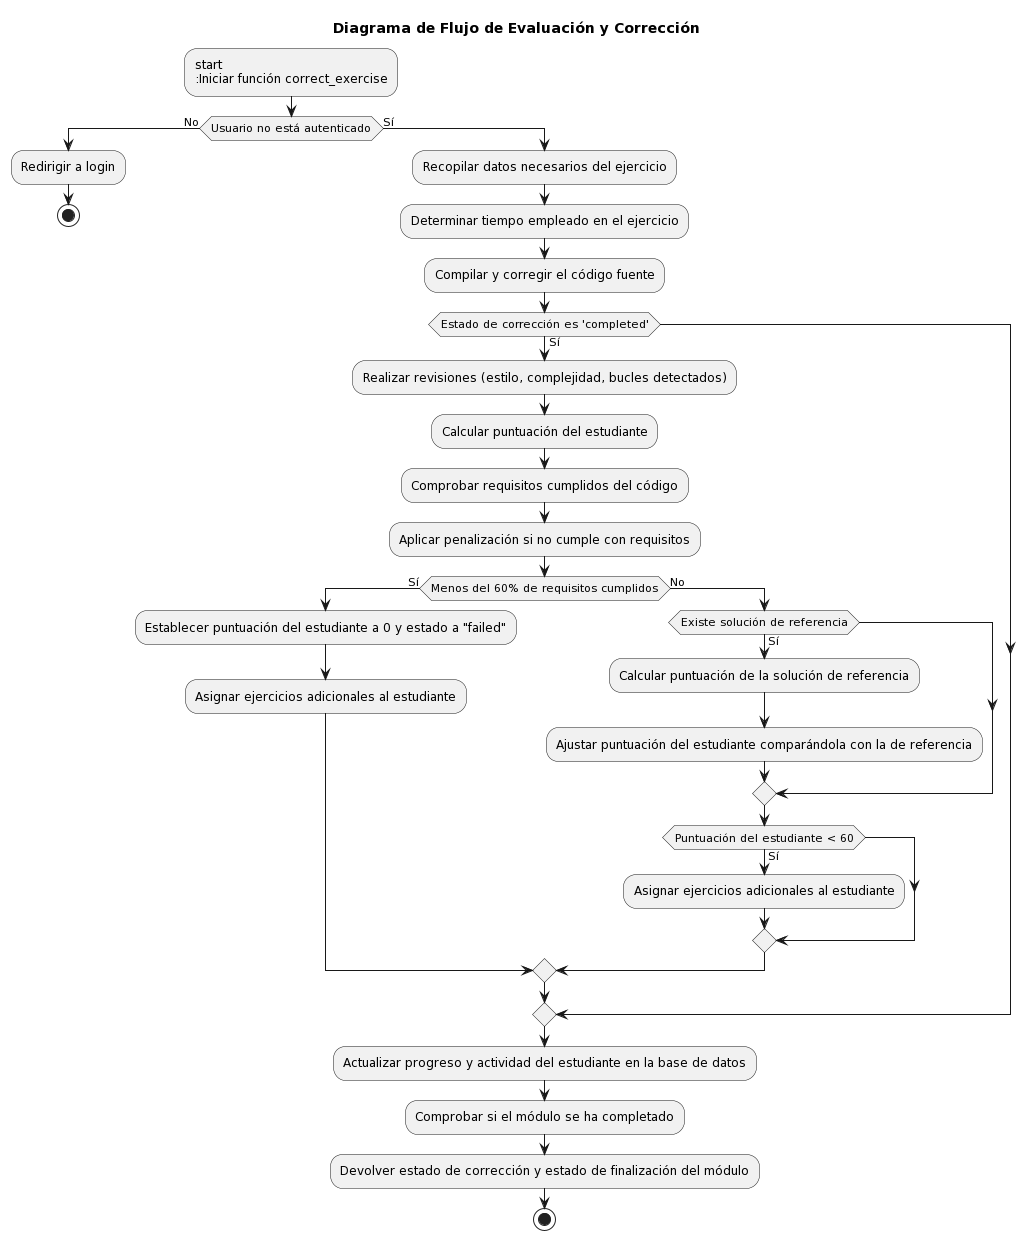
\includegraphics[width=\textwidth]{imagenes/correcionejercicios.png}
    \caption{Diagrama de flujo para la selección de ejercicios}
    \label{fig:correccion}
    \end{figure}

\subsection{Algoritmo para la selección y evaluación de ejercicios}

El sistema prioriza la progresión estructurada del estudiante. Al ingresar, la plataforma identifica ejercicios en curso o determina el próximo paso en función de los requisitos del módulo. Esta estructura garantiza que, antes de enfrentarse a cualquier tarea, los conceptos teóricos relevantes sean presentados al estudiante \ref{fig:seleccion}. Esta estrategia se fundamenta en la pedagogía moderna, que sugiere que la teoría y la práctica deben ir de la mano para un aprendizaje óptimo.

\begin{figure}[H]
\centering
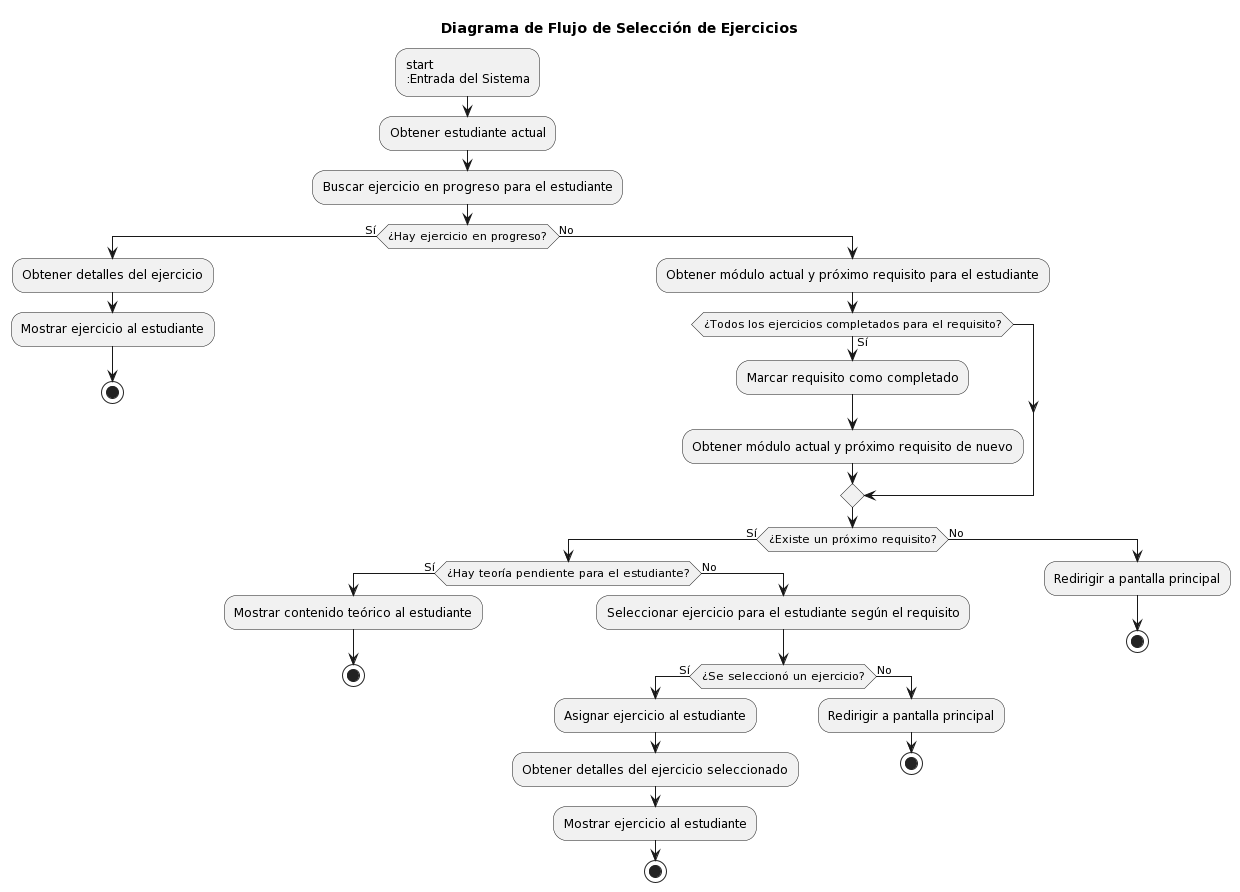
\includegraphics[width=\textwidth]{imagenes/seleccionejercicios.png}
\caption{Diagrama de flujo para la selección de ejercicios}
\label{fig:seleccion}
\end{figure}

\section{Tecnologías y Herramientas}
Enumere las tecnologías, lenguajes de programación, frameworks y bibliotecas utilizadas.

\section{Implementación de Módulos de Aprendizaje Adaptativo}
Describa cómo el sistema se adapta al progreso del estudiante.


    % Analisis de resultados
    \chapter{Despliegue} \label{chap:despliegue}

En este capítulo se va a abordar el despliegue de la aplicación Flask en el servidor de la Universidad de Granada \textit{bahia.ugr.es} \cite{bahia}. Concretamente, el despliegue se llevó a cabo mediante Podman \cite{podman} para la gestión de los contenedores. A continuación, se detallará el proceso de creación y configuración de las imágenes del contenedor, así como la metodología empleada.

\section{Creación y Configuración de las Imágenes}

Las imágenes del contenedor creadas fueron:

\begin{itemize}
    \item \textbf{Imagen de la aplicación}: Se creó una imagen personalizada para la aplicación Flask, etiquetada como \texttt{nooocaaaa/programmingclasses: latest} \ref{fig:dockerfileapp}. Esta imagen incorpora todas las dependencias necesarias para la ejecución de la aplicación, así como las configuraciones específicas requeridas. La imagen fue construida utilizando Docker y posteriormente subida a Docker Hub \cite{dockerhub}, facilitando su distribución y posterior acceso. 
    \item \textbf{Imagen de la base de datos}:  De forma análoga, se generó una imagen personalizadapara el servidor de base de datos PostgreSQL, etiquetada como \texttt{nooocaaaa/postgres-tfg:latest} \ref{fig:dockerfilebbdd}. Esta imagen está optimizada para integrarse con la aplicación Flask y también está disponible en Docker Hub \cite{dockerhub2}.
\end{itemize}

\section{Utilización de Podman}

A partir de un archivo \texttt{docker-compose.yml} \ref{fig:dockercompose}, testeado en \textit{localhost}, se adapto la configuración para su uso con Podman. De esta manera, se aprovechó la compatibilidad y las ventajas de seguridad de esta herramienta, especialmente en entornos donde no se tienen privilegios de root.

En la configuración del fichero \texttt{podman-compose.yml} \ref{fig:podmancompose}, se establecieron dos servicios principales: el servicio de la aplicación (flask) y el servicio de la base de datos (db). Cada uno de estos servicios se configuró cuidadosamente para garantizar una integración y operación eficientes. 

Esta configuración facilitó un despliegue coherente y funcional de la aplicación en el entorno de Podman, proporcionando un marco de trabajo estable y confiable para el funcionamiento de la aplicación Flask y su interacción con la base de datos PostgreSQL.

\subsection{Contenedor flask\_TFG}

El servicio Flask se configuró con el nombre de contenedor \texttt{flask\_TFG}, utilizando la imagen \texttt{nooocaaaa/programmingclasses:latest} anteriormente mencionada. Esta imagen, especialmente diseñada para la aplicación, contiene todas las dependencias y configuraciones necesarias. 

Se mapeó el puerto \texttt{35701} del host al contenedor, proporcionando un punto de acceso a la aplicación para la comunicación con el exterior. Las variables de entorno se establecieron para configurar la conexión con la base de datos, definir claves secretas y especificar rutas de directorios críticos. Además, se definió una dependencia con el servicio de base de datos para asegurar que la base de datos estuviera disponible antes del inicio de la aplicación Flask. Es más, el comando de ejecución para el contenedor se configuró para iniciar la aplicación Flask.

\subsection{Contenedor db}

Por otro lado, el servicio de base de datos, etiquetado como \texttt{db}, utilizó la imagen \texttt{nooocaaaa/postgres-tfg:latest}, optimizada para trabajar en conjunto con la aplicación Flask.

Se expuso el puerto \texttt{5432} para permitir la comunicación con la base de datos. Las variables de entorno se configuraron para establecer los parámetros de la base de datos, incluyendo el nombre de la base de datos, el usuario y la contraseña. Para garantizar la persistencia de los datos, se utilizó un volumen, con tal que los datos se mantengan seguros y accesibles incluso después de reiniciar o detener el contenedor.



    % Analisis de resultados
    \chapter{Pruebas y Resultados} \label{chap:resultadosExperimentales}

Este capítulo se centra en análisis de las pruebas realizadas para evaluar la efectividad y eficiencia del sistema desarrollado. Estas pruebas se clasifican en tres categorías principales. Cada una de estas pruebas juega un papel crucial en la validación del sistema, asegurando que cumple con los requisitos establecidos y proporciona una experiencia de usuario satisfactoria. Los resultados obtenidos no solo demuestran la viabilidad del sistema, sino que también ofrecen \textit{insights} valiosos para futuras mejoras y ajustes.

\section{Pruebas de Funcionalidad}

Esta sección se centra en las diferentes pruebas de funcionalidad realizadas para garantizar la calidad y el correcto funcionamiento del sistema. Estas pruebas incluyen diferentes tipos de prueba, ya que cada una de ellas dirigida a validar aspectos específicos de la plataforma.

\subsection{Pruebas Unitarias}

Las pruebas unitarias se enfocaron en validar la funcionalidad de los componentes individuales del sistema. Concretamente, se escribieron casos de prueba para cada función y método, cubriendo tanto los escenarios esperados como los casos extremos. Se validaron las salidas de cada componente para garantizar que cumplieran con las especificaciones y requisitos funcionales. Se prestó especial atención a la cobertura de código, buscando lograr un porcentaje alto que garantice la fiabilidad del sistema.

\subsection{Pruebas de Integración}

Las pruebas de integración se centraron en la interacción entre los componentes individuales del sistema para asegurar que funcionaran juntos de manera efectiva.

Se probaron las interfaces y las interacciones entre diferentes módulos y servicios. Se realizaron pruebas de llamadas a APIs, interacción con bases de datos y comunicación entre servicios. Se identificaron y corrigieron problemas de integración, como incompatibilidades y fallos en la transferencia de datos con la ayuda de Postman \cite{postman}. 

\subsection{Pruebas Manuales}
Las pruebas manuales fueron cruciales para validar la experiencia del usuario y la funcionalidad desde una perspectiva más humana. Se llevaron a cabo sesiones de prueba donde se interactuaba con la aplicación de manera natural, buscando errores o problemas de usabilidad. Se observó el comportamiento de la aplicación en diferentes dispositivos y sistemas operativos para asegurar su compatibilidad y adaptabilidad. Se realizaron pruebas de escenarios de usuario, simulando diferentes flujos de trabajo y operaciones comunes.

\subsection{Pruebas de Navegación y Flujo de Usuario}

Estas pruebas se enfocaron en la experiencia del usuario al navegar por la aplicación y realizar tareas específicas, asegurando una interfaz intuitiva y eficiente. Se evaluó la lógica y coherencia de la interfaz de usuario, asegurando que los flujos de trabajo fueran claros y fáciles de seguir. Se prestó atención a la experiencia del usuario al completar tareas comunes, buscando minimizar la complejidad y maximizar la eficiencia.

En resumen, las pruebas de funcionalidad jugaron un papel fundamental en la validación y mejora continua del sistema, asegurando que cumpliera con los requisitos funcionales y proporcionara una experiencia de usuario satisfactoria antes de la prueba con niños.


\section{Pruebas de Rendimiento}

Las pruebas de rendimiento se llevaron a cabo para evaluar la capacidad del sistema para manejar cargas de trabajo significativas y para identificar cualquier posible cuello de botella. Se utilizaron escenarios de prueba que reflejaban el uso típico del sistema por parte de los usuarios finales.

Se empleó Apache JMeter \cite{jmeter}, una herramienta de prueba de carga de código abierto, para simular múltiples solicitudes al servidor, con el fin de imitar el comportamiento de varios usuarios accediendo al sistema simultáneamente. 

La configuración de JMeter se ajustó para incrementar gradualmente el número de usuarios virtuales y generar una carga significativa en el servidor.

\subsection{Configuración de la Prueba}

La configuración de la prueba incluyó:

\begin{itemize}
    \item Número total de peticiones: 10,000
    \item Usuarios concurrentes (hilos): 1,000
    \item Duración de la prueba: 10 minutos
    \item Tiempo de rampa: 100 segundos
\end{itemize}

\subsection{Resultados Observados}

Los resultados de las pruebas mostraron que el sistema era capaz de manejar un throughput de 96.92 peticiones por minuto con una variabilidad en los tiempos de respuesta. Los tiempos de respuesta promedio se mantuvieron en 44 ms, con una mediana de 12 ms, lo que indica una respuesta rápida bajo carga para la mayoría de los usuarios.

\begin{figure}[H]
\centering
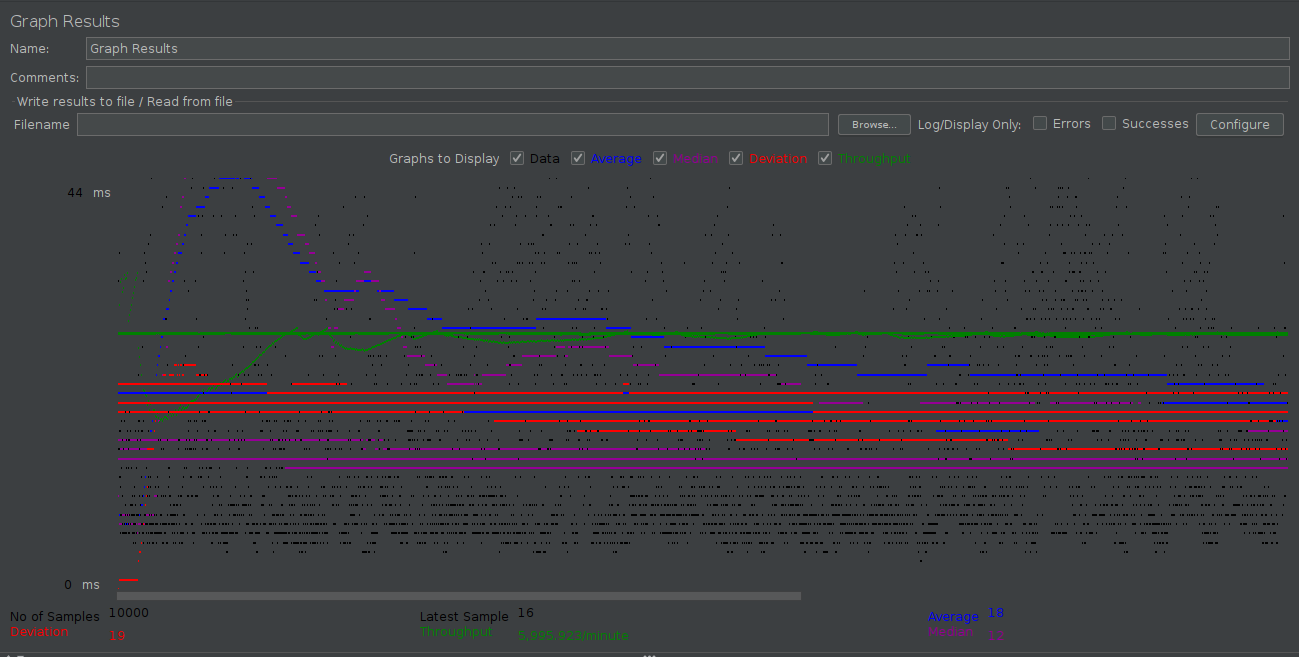
\includegraphics[width=\textwidth]{imagenes/graforendimiento.png}
\caption{Resultados gráficos de la prueba de rendimiento con JMeter.}
\label{fig:grafico-jmeter}
\end{figure}

Los datos recogidos sugieren que la experiencia del usuario se mantendría consistente hasta cierto punto de carga. Sin embargo, se observaron advertencias relacionadas con la gestión de cookies, lo que podría ser un indicador de problemas de configuración en el manejo de sesiones de usuario o en el estado del sistema.

El análisis de los resultados recogidos sugiere que el sistema es robusto y puede manejar cargas de usuarios concurrentes de manera efectiva hasta un punto crítico. Cumpliendo, de esta manera, el requisito \ref{table:req-RNF38} del tiempo de respuesta establecido en la fase de análisis del proyecto.

\section{Pruebas de Usabilidad}

Con el fin de evaluar correctamente el sistema implementado, también se realizaron pruebas con un pequeño pero significativo grupo de niños, compuesto por 3 participantes de distintas edades. Concretamente de 8, 12 y 15 años. Cada uno de ellos interactuó con el sistema de manera individual, en sesiones separadas. De esta manera, se obtuvo una evaluación más detallada y precisa de la eficacia del sistema.

Las tareas asignadas para las pruebas en la página web incluyeron (véase anexo \ref{chap:guion}):

\begin{itemize}
    \item Navegación por el sitio y localización de información específica.
    \item Resolución de ejercicios de programación y lógica.
    \item Cuestionario oral sobre la lectura de contenidos de teoría o enunciados de ejercicios.
\end{itemize}

Los indicadores cuantitativos mostraron resultados bastante alentadores. Se registró el tiempo en la tabla \ref{tab:pruebast} donde se puede visualizar el tiempo que cada participante empleó en completar las tareas asignadas:

\begin{table}[h]
\centering
\begin{tabular}{|c|c|c|c|}
\hline
Edad   & Navegación (min) & Ejercicios (min) & Cuestionario (min) \\ \hline
8 años & 14              & 23               & 22                 \\ \hline
12 años & 10              & 15               & 12                 \\ \hline
15 años & 6               & 14              & 10                 \\ \hline
\end{tabular}
\caption{Tiempo empleado en tareas por edad}
\label{tab:pruebast}
\end{table}

Los jóvenes usuarios lograron completar los ejercicios con éxito. Además, el tiempo que pasaron interactuando con la plataforma se mantuvo en un rango óptimo. Por lo tanto, se puede decir que el sistema fue eficaz en adaptarse a la dificultad. Sin embargo, se observó que el tiempo óptimo de interacción con el sistema debería ajustarse según la edad del usuario, dado que las capacidades de atención y ritmo de lectura varían considerablemente en función de la edad. 

En términos de usabilidad, las respuestas fueron positivas. La plataforma fue calificada como fácil de usar y práctica, lo cual indica que el diseño de la interfaz es adecuado. La claridad en las instrucciones también fue un punto destacado aunque a veces desconcertante para los más pequeños debido a su capacidad de distracción.

Entre las sugerencias aportadas, la más recurrente fue la adición de elementos como juegos con tal de incrementar la motivación y el compromiso. Este tipo de retroalimentación fue especialmente valiosa y se consideró como una mejora importante a realizar en el sistema. Además, la metodología de pruebas individuales permitió recoger opiniones y sugerencias sin la influencia o presión del grupo.

En conclusión, las pruebas iniciales sugirieron que el sistema era efectivo en su misión de ofrecer una experiencia de aprendizaje adaptativo. Los comentarios y observaciones de los jóvenes participantes ofrecieron un conjunto invaluable de datos que sirvieron para enriquecer el sistema.


     % Conclusiones
    \chapter{Conclusiones y Trabajo Futuro} \label{chap:conclusiones}

Este último capítulo sirve como el cierre al Trabajo de Fin de Grado presentado. En él, se busca sintetizar los hallazgos más significativos, destacando cómo estos contribuyen al campo de la enseñanza de la programación a niños. Asimismo, se esbozarán las direcciones para el trabajo futuro, delineando oportunidades para la expansión. Finalmente, se ofrecerá una reflexión personal sobre el impacto del proyecto.

\section{Conclusiones}

Este TFG se ha centrado en un reto: la enseñanza de la programación a niños en un contexto de una sociedad digitalizada en rápida evolución. A través de un enfoque multidisciplinario combinando pedagogía, tecnología educativa y diseño de sistemas (veáse capítulo \ref{chap:stateoftheart},), se ha desarrollado una plataforma adaptable dentro del campo de la enseñanza cumpliendo así los objetivos establecidos.

Un logro clave ha sido el desarrollo del Sistema de Tutorización Inteligente, que supera las barreras de algunos de los métodos tradicionales al ofrecer un aprendizaje personalizado y adaptativo. Este sistema no solo puede mejorar la calidad del aprendizaje, sino que también puede permitir a los estudiantes progresar a su propio ritmo.

La colaboración con Codelearn S.L. ha sido instrumental, fusionando teoría y práctica para evaluar y mejorar el ITS, y así dar los primeros pasos hacia un sistema educativo más eficaz y atractivo para los jóvenes de hoy en día.

\section{Trabajo Futuro}

El proyecto, aunque completo, es el principio de un camino amplio. La colaboración con Codelearn S.L. no solo ha demostrado la viabilidad del proyecto, sino que también ha abierto puertas para su continuación y expansión. Los siguientes pasos están alineados con la visión y estrategia a largo plazo de la empresa, asegurando que el trabajo realizado tenga un impacto duradero y evolutivo.

\begin{itemize}
    \item \textbf{Variedad de Recursos Didácticos}: Una mayor diversidad en el tipo de ejercicios y evaluaciones, cómo relleno de huecos de un código o cuestionarios sobre ciertos temas, entre otros ejemplos.
    \item \textbf{Automatización  de la Corrección}: Conseguir automatizar la corrección para los ejercicios HTML y que no se recurra a la figura del profesor para ello. 
    \item \textbf{Sistema de Chat-Bot}: Sistema conversacional para una primera resolución de dudas comunes en un ejercicio, como una explicación más extensa o ejemplos de ejecución.  
    \item \textbf{Inteligencia Artificial}: El uso de algoritmos de aprendizaje automático que optimizaría la adaptabilidad del sistema a las necesidades individuales del estudiante, debido a la gran cantidad de datos con la que entrenaría.
    \item \textbf{Feedback en Tiempo Real}: La implementación de análisis del código mientras el estudiante lo este escribiendo con tal de poder hacer ajustes o los comentarios pertinentes.
    \item \textbf{Tests A/B}: Realización de pruebas para evaluar la eficacia de distintas técnicas pedagógicas y elementos de diseño.
  \end{itemize}

\section{Reflexión Personal}
Desde la concepción inicial del proyecto hasta la implementación técnica y las pruebas finales, cada etapa ha contribuido a un desarrollo profesional.

Empezando con la colaboración con Codelearn S.L., la experiencia ha sido invaluable. Ver un entorno real me ha ofrecido perspectivas que el ámbito académico raramente puede proporcionar. He aprendido a abordar problemas desde un punto de vista más aplicado, equilibrando teoría y práctica. Fortaleciendo, así, mi comprensión sobre cómo llevar soluciones tecnológicas desde el tablero de dibujo hasta una implementación funcional y real.

En el aspecto académico, este proyecto ha servido como una especie de trampolín para relacionar la ingeniería de software, los algoritmos y la pedagogía. Ganando una visión más clara de cómo la mayoría de disciplinas se pueden fusionar para producir soluciones educativas efectivas. 

El desarrollo ágil adoptado para el proyecto fue una lección valiosa en sí misma. Me enseñó la importancia de la adaptabilidad y la agilidad en un entorno tecnológico que nunca se detiene. La retroalimentación continua y los ajustes constantes fueron cruciales para navegar a través de los desafíos que inevitablemente surgieron.



    \newpage
    \appendix
    \addcontentsline{toc}{chapter}{Anexos}
    \begin{appendices}

\chapter{Recursos Informáticos} \label{chap:recursos}

En este apéndice se detalla todos los recursos de hardware y software que se han usado durante la ejecución de este proyecto. Esta información es esencial para entender el entorno de desarrollo y ejecución, permitiendo así una mejor replicación o continuación del trabajo realizado.
    
\section{Hardware}

Para el desarrollo y ejecución de este proyecto, se ha utilizado el siguiente hardware:

\begin{itemize}
    \item Ordenador portátil \textit{Xiaomi TM1703}.
    \begin{itemize}
    \item Arquitectura de 64 bits.
    \item 8 GB de Memoria RAM.
    \item Procesador \textit{ Intel(R) Core(TM) 5-8250U CPU @ 1.60GHz}.
    \end{itemize}
\end{itemize}

\section{Software}

En cuanto al software, se han utilizado las siguientes herramientas y plataformas:

\begin{itemize}
    \item \textbf{Sistema Operativo}: Ubuntu 20.04.6 LTS.
    \item \textbf{Contenedores}: Docker, versión 24.0.5.
    \item \textbf{IDE}: Visual Studio Code 1.83.1
    \item \textbf{Base de datos}: PostgreSQL 16.0
    \item \textbf{Lenguaje de programación}: Python 3.8.10
    \item \textbf{Procesador de textos}: LaTex 3.14159265-2.6-1.40.20
    \item \textbf{Diseño de E-R}: draw.io
    \item \textbf{Modelado de datos}: PostgreSQL 16.0
    \item \textbf{Diagrama de flujo y arquitectura}: PlantUML v1.2023.12
    \item \textbf{Mockups}: Wireframe.cc
    \item \textbf{Bibliotecas Python}:
    \begin{itemize}
        \item Flask \cite{flask}
        \item Flask-Login \cite{flask-login}
        \item Flask-SQLAlchemy \cite{flask-sqlalchemy}
        \item Flask-CORS \cite{flask-cors}
        \item Flask-Bcrypt \cite{flask-bcrypt}
        \item python-dotenv \cite{python-dotenv}
        \item datetime \cite{datetime}
        \item werkzeug.utils \cite{werkzeug}
        \item radon.complexity \cite{radon}
    \end{itemize}
\end{itemize}
    
\chapter{Guion pruebas con niños}

Este guion tiene como objetivo guiar las pruebas de la plataforma de programación para niños. Se busca evaluar la usabilidad, el interés generado y la eficacia educativa del sistema.

\section{Preparación}
\begin{itemize}
    \item Preparar un ambiente tranquilo y sin distracciones.
    \item Asegurarse de que la plataforma funcione correctamente.
    \item Tener a mano material para tomar notas.
\end{itemize}

\section{Participantes}
\begin{itemize}
    \item Edades entre 7 y 18 años.
    \item Con y sin experiencia previa en programación.
\end{itemize}

\section{Actividades}
\subsection*{Introducción y Consentimiento}
\begin{itemize}
    \item Explicar el objetivo de la prueba.
\end{itemize}

\subsection*{Prueba de Usabilidad}
\begin{itemize}
    \item Navegar por la plataforma.
    \item Completar un ejercicio.
    \item Utilizar las herramientas de ayuda o tutoriales, si están disponibles.
\end{itemize}

\subsection*{Prueba de Interés}
\begin{itemize}
    \item Observar las reacciones de los niños mientras usan la plataforma.
    \item Preguntarles qué les gusta y qué no.
\end{itemize}

\subsection*{Prueba de Eficacia Educativa}
\begin{itemize}
    \item Evaluar el conocimiento adquirido con un pequeño cuestionario oral.
\end{itemize}

\section{Feedback y Conclusiones}
\begin{itemize}
    \item Pedir a los niños que proporcionen comentarios.
    \item Analizar los resultados y planificar mejoras para la plataforma.
\end{itemize}


\chapter{Manual de uso de la Plataforma}

\end{appendices}
    \newpage
    \section*{Glosario}

\begin{description}
    \item[ITS:] Sistema Inteligente de Tutorización (Intelligent Tutoring System). Es un sistema que utiliza tecnologías de inteligencia artificial para proporcionar enseñanza personalizada y apoyo educativo a los estudiantes, adaptándose a las necesidades individuales de aprendizaje.
    \item[Hash y Salting:] Técnicas de seguridad para el almacenamiento seguro de contraseñas. El "hashing" convierte una contraseña en una cadena de caracteres única, mientras que "salting" añade datos aleatorios al hash para aumentar la seguridad.
    \item[HTTPS:] Protocolo seguro para la transferencia de datos en la web. Utiliza el protocolo SSL/TLS para encriptar la información transmitida.
    \item[Flujo:] Secuencia de pasos o actividades en un proceso o escenario. En el contexto de programación, se refiere a la ejecución ordenada de instrucciones en un programa.
    \item[Web Responsive:] Diseño web adaptable a diferentes dispositivos. Utiliza hojas de estilo en cascada (CSS) para ajustar el diseño según el tamaño de la pantalla.
    \item[Gamificación:] Uso de elementos de juego en entornos no lúdicos. Se emplea para aumentar la motivación y la participación en actividades que normalmente se considerarían tediosas.
    \item[Aprendizaje Basado en Problemas (ABP):] Método pedagógico que utiliza problemas reales o simulados como punto de partida para el aprendizaje.
    \item[API RESTful:] Interfaz de programación de aplicaciones que sigue los principios REST para la comunicación entre sistemas.
    \item[Backend:] Parte del sistema que se encarga de la lógica de negocio, el acceso a la base de datos y la comunicación con diferentes servicios.
    \item[Clave Primaria:] Campo único en una tabla de base de datos que se utiliza para identificar registros de forma única.
    \item[Clave Foránea:] Campo en una tabla de base de datos que se utiliza para establecer una relación con otra tabla.
    \item[Normalización:] Proceso de organización de una base de datos para reducir la redundancia y mejorar la integridad de los datos.
    \item[Análisis de Árbol de Sintaxis Abstracta (AST):] Técnica de análisis de código que genera un árbol para representar su estructura sintáctica.
    \item[Complejidad Ciclomática:] Métrica que mide la complejidad de un programa basada en el número de caminos independientes a través del código.
    \item[Función Indicadora:] Función matemática que toma el valor de 1 si una condición específica se cumple y 0 en caso contrario.
    \item[Requisitos de Aprendizaje:] Objetivos educativos específicos que un estudiante debe alcanzar en un sistema de aprendizaje adaptativo.
    \item[Tasa de Fracaso:] Proporción de ejercicios o tareas que un estudiante no ha podido completar con éxito.
    \item[Normalización:] Proceso de ajustar valores medidos en diferentes escalas a una escala común.
    \item[Ponderación:] Asignación de importancia relativa a diferentes criterios o variables en un cálculo.
    \item[Análisis Estático:] Examinar el código en busca de problemas sin ejecutar el programa.
    \item[Adaptabilidad:] Capacidad de un sistema para ajustarse dinámicamente a las necesidades o comportamientos del usuario.
    \item[Fitness:] Métrica que evalúa la calidad o eficacia de una solución en comparación con una solución de referencia.
    \item[Indicadores Cuantitativos:] Métricas numéricas utilizadas para evaluar el rendimiento o eficacia de un sistema.
    \item[Usabilidad:] Medida de la eficacia, eficiencia y satisfacción con la que los usuarios pueden realizar tareas en un sistema.
    \item[Metodología de Pruebas Individuales:] Enfoque de evaluación que implica probar el sistema con cada usuario de forma separada para obtener retroalimentación más precisa.
    \item[Optimización:] Proceso de hacer cambios en un sistema para mejorarlo en términos de eficiencia, eficacia o experiencia del usuario.
\end{description}

    \addcontentsline{toc}{chapter}{Glosario}
    \printglossary
    \bibliographystyle{plain} 
    \bibliography{Bibliografia/referencias}  \label{bibliografia}
    \addcontentsline{toc}{chapter}{Bibliografía}
    \newpage



\end{document}
